\documentclass{article}%
\usepackage[T1]{fontenc}%
\usepackage[utf8]{inputenc}%
\usepackage{lmodern}%
\usepackage{textcomp}%
\usepackage{lastpage}%
%
\usepackage{amsmath}%
\usepackage{amssymb}%
\usepackage{amsfonts}%
\usepackage{graphicx}%
\usepackage{hyperref}%
\usepackage{tikz}%
\usepackage{pgfplots}%
\usetikzlibrary{math}%
\title{ITA 2027 - Física\thanks{This exam was solved and automatically generated with gpt-resolve: \url{https://github.com/lgabs/gpt-resolve}}}%
\author{claude{-}haiku{-}5{-}5 (solver) + claude{-}haiku{-}5{-}5 (judge)}%
\date{November 09, 2026}%
%
\begin{document}%
\normalsize%
\maketitle%
\section*{Questão 1}

\section*{Solução}

\textbf{Modelo e hipóteses.} A haste (massa $M$, comprimento $L$, homogênea) gira num plano vertical em torno do eixo fixo $O$, sua extremidade inferior, que coincide com o eixo do corpo de prova. Os únicos torques são o do peso e o elástico, $\tau_e=-k\theta$; o atrito nos mancais é desprezado. Hipóteses: movimento plano; centro de massa (CM) no ponto médio, a $L/2$ de $O$; $\theta$ medido a partir da vertical, positivo no sentido horário da figura; aquecimento lento, de modo que $k$ é constante em cada instante e o sistema segue os equilíbrios (quase estático). Como o corpo de prova está fixo nos mancais, a altura $h_O$ de $O$ acima do mancal é constante.

\textbf{Equação do movimento.} Pelo teorema dos eixos paralelos, $I_O=\frac{ML^2}{12}+M\left(\frac{L}{2}\right)^2=\frac{ML^2}{3}$. O peso tem braço $\frac{L}{2}\operatorname{sen}\theta$ e, como o CM está acima de $O$ para $|\theta|<\pi/2$, seu torque tende a aumentar $|\theta|$ (pêndulo invertido). Pela segunda lei para rotação em torno de eixo fixo, $\sum\tau_O=I_O\,\ddot\theta$:
\[
\frac{ML^2}{3}\,\ddot{\theta}=\frac{MgL}{2}\operatorname{sen}\theta-k\theta. \tag{1}
\]

\textbf{Energia potencial.} Os torques conservativos são $-k\theta=-\frac{d}{d\theta}\left(\frac{1}{2}k\theta^2\right)$ e $\frac{MgL}{2}\operatorname{sen}\theta=-\frac{d}{d\theta}\left[\frac{MgL}{2}\cos\theta\right]$. Com a energia gravitacional $Mg\,y_{CM}$, sendo $y_{CM}=h_O+\frac{L}{2}\cos\theta$ a altura do CM medida a partir do mancal,
\[
U_{total}(\theta)=\frac{1}{2}k\theta^2+Mg\left(h_O+\frac{L}{2}\cos\theta\right)+C.
\]
A constante $C$ é arbitrária (escolha de referência) e não altera $dU_{total}/d\theta$ nem $d^2U_{total}/d\theta^2$; tomamos $C=0$. $U_{total}$ é apenas potencial: a energia cinética $\frac{ML^2}{6}\dot\theta^2$ não entra nela. Assim, (1) equivale a $\frac{ML^2}{3}\ddot\theta=-\frac{dU_{total}}{d\theta}$.

\textbf{Equilíbrio e estabilidade.} Um equilíbrio $\theta^*$ é um estado de repouso ($\dot\theta=0$) com $\ddot\theta=0$, isto é, $\frac{dU_{total}}{d\theta}(\theta^*)=0$. Para um desvio pequeno $\delta=\theta-\theta^*$, $\frac{ML^2}{3}\ddot\delta=-U_{total}''(\theta^*)\,\delta$: se $U_{total}''(\theta^*)>0$ há oscilação e o equilíbrio é estável; se $U_{total}''(\theta^*)<0$, o desvio cresce e o equilíbrio é instável; se $U_{total}''(\theta^*)=0$, o teste linear é inconclusivo.

\textbf{a)} Com $\operatorname{sen}\theta\approx\theta$ para $\theta\ll 1$, (1) fica
\[
\frac{ML^2}{3}\,\ddot{\theta}=-\left(k-\frac{MgL}{2}\right)\theta,
\]
ou seja, $U_{total}''(0)=k-\frac{MgL}{2}$. Se $k>\frac{MgL}{2}$, $\omega^2=\frac{3}{ML^2}\left(k-\frac{MgL}{2}\right)>0$ e há oscilação em torno de $\theta=0$ (estável). Se $k<\frac{MgL}{2}$, $\ddot\theta$ tem o mesmo sinal de $\theta$ e o desvio cresce exponencialmente (instável). Portanto
\[
k_C=\frac{MgL}{2}.
\]
Conferências: $[MgL]=\mathrm{N\,m}$ e $[k]=\mathrm{N\,m/rad}=\mathrm{N\,m}$, pois o radiano é adimensional. A inércia não aparece em $k_C$; ela entra só na frequência, $\omega^2=\frac{3g}{2L}\left(\frac{k}{k_C}-1\right)$. Para $k=0$ a taxa de crescimento é $\sqrt{3g/(2L)}$, o resultado conhecido de uma haste uniforme articulada na extremidade. Em $k=k_C$ o teste linear é inconclusivo; o item b mostra que a vertical ainda é estável nesse valor, por isso o enunciado fala em $k<k_C$.

\textbf{b)} Seja $\lambda=k/k_C>0$, com $k=\lambda\frac{MgL}{2}$. Então
\[
\frac{dU_{total}}{d\theta}=k_C\left(\lambda\theta-\operatorname{sen}\theta\right),\qquad \frac{d^2U_{total}}{d\theta^2}=k_C\left(\lambda-\cos\theta\right).
\]
O ponto $\theta=0$ é sempre equilíbrio. Os demais satisfazem $f(\theta)=\lambda$, com $f(\theta)=\frac{\operatorname{sen}\theta}{\theta}$, função par com $f(0)=1$ por limite.

Seja $g(\theta)=\theta\cos\theta-\operatorname{sen}\theta$. Como $g(0)=0$ e $g'(\theta)=-\theta\operatorname{sen}\theta<0$ para $0<\theta<\pi$, tem-se $g<0$ nesse intervalo e $f'(\theta)=\frac{g(\theta)}{\theta^2}<0$. Logo $f$ decresce estritamente de $1$ (com $\theta\to0^+$) até $0$ (em $\theta=\pi$), passando por $f(\pi/2)=\frac{2}{\pi}$. Pelo teorema do valor intermediário e pela monotonia estrita:
\begin{itemize}
\item se $0<\lambda<1$, há exatamente uma raiz $\theta^*\in(0,\pi)$; ela está em $(0,\pi/2)$ se $\lambda>\frac{2}{\pi}$, vale $\pi/2$ se $\lambda=\frac{2}{\pi}$ e está em $(\pi/2,\pi)$ se $\lambda<\frac{2}{\pi}$;
\item se $\lambda\ge 1$, não há raiz em $(0,\pi)$, pois $\operatorname{sen}\theta<\theta$ para $\theta>0$.
\end{itemize}
Por paridade, $-\theta^*$ também é raiz. Assim, em $(-\pi/2,\pi/2)$ existem raízes não nulas se e somente se $\frac{2}{\pi}<\lambda<1$; são $\pm\theta_e$, com $0<\theta_e<\pi/2$, únicas pela monotonia.

\textit{Natureza.} Em $\theta=0$, $U_{total}''(0)=k_C(\lambda-1)$. Em $\pm\theta_e$, usando $\lambda=\frac{\operatorname{sen}\theta_e}{\theta_e}$,
\[
U_{total}''(\pm\theta_e)=k_C\left(\frac{\operatorname{sen}\theta_e}{\theta_e}-\cos\theta_e\right)=-k_C\,\frac{g(\theta_e)}{\theta_e}>0,
\]
logo $\pm\theta_e$ são mínimos locais, estáveis. A raiz $\theta^*\in(\pi/2,\pi)$, quando existe, tem $\cos\theta^*<0<\lambda$, logo $U_{total}''>0$: também estável, mas fora do intervalo pedido. Os casos são:
\begin{enumerate}
\item $\frac{k}{k_C}>1$: não há raiz não nula. Único equilíbrio, $\theta=0$, \textbf{estável}, pois $U_{total}''(0)>0$.
\item $\frac{k}{k_C}=1$: não há raiz não nula. O teste linear é inconclusivo, mas $\frac{dU_{total}}{d\theta}=k_C(\theta-\operatorname{sen}\theta)$ tem o sinal de $\theta$; logo $\theta=0$ é mínimo global estrito no intervalo: \textbf{estável} (degenerado), com $U_{total}-U_{total}(0)\approx\frac{MgL}{48}\theta^4$.
\item $\frac{2}{\pi}<\frac{k}{k_C}<1$: $\theta=0$ é \textbf{instável} ($U_{total}''(0)<0$) e há três equilíbrios: $\theta=0$ instável e $\pm\theta_e$ \textbf{estáveis}, com $\frac{\operatorname{sen}\theta_e}{\theta_e}=\frac{k}{k_C}$.
\item $0<\frac{k}{k_C}\le\frac{2}{\pi}$: no intervalo aberto resta só $\theta=0$, \textbf{instável}. Para $\frac{k}{k_C}<\frac{2}{\pi}$ existe um equilíbrio estável $\theta^*\in(\pi/2,\pi)$, fora do intervalo; para $\frac{k}{k_C}=\frac{2}{\pi}$ ele está exatamente na borda $\theta=\pi/2$, também excluída.
\end{enumerate}

\textit{Evolução física.} Ao aquecer, $k$ diminui. Para $k>k_C$ a vertical é o único equilíbrio e é estável. Em $k=k_C$ ocorre bifurcação em forquilha: a vertical perde estabilidade e os ramos $\pm\theta_e$ nascem continuamente dela (perto de $\lambda=1$, $f\approx 1-\frac{\theta^2}{6}$ dá $\theta_e\approx\sqrt{6(1-\lambda)}$). Como o aquecimento é lento, a haste acompanha o ramo estável, cujo ângulo cresce até $\pi/2$ em $k=\frac{2}{\pi}k_C$, quando fica horizontal. O modelo é simétrico por $\theta\mapsto-\theta$ e não escolhe o sinal: a haste vai para $+\theta_e$ ou $-\theta_e$ conforme imperfeições de montagem ou perturbações. Com simetria perfeita, $\theta=0$ continuaria equilíbrio, mas instável. Abaixo de $\frac{2}{\pi}k_C$ não há equilíbrio no intervalo, e a haste tende a passar da horizontal até $\theta^*$, continuação do mesmo ramo.

\textbf{c)} Com $\lambda=k/k_C$, $\frac{1}{2}k\theta^2=\frac{MgL}{2}\cdot\frac{\lambda\theta^2}{2}$, logo
\[
U_{total}(\theta)=Mg\,h_O+\frac{MgL}{2}\left[\cos\theta+\frac{\lambda}{2}\,\theta^2\right].
\]
A constante $Mg\,h_O$ apenas desloca o gráfico. $U_{total}$ é par, então basta analisar $(0,\pi/2)$, usando o sinal de $\frac{dU_{total}}{d\theta}=k_C(\lambda\theta-\operatorname{sen}\theta)$ e de $U_{total}''$.
\begin{itemize}
\item (i) $\lambda>1$: para $\theta>0$, $\lambda\theta>\theta>\operatorname{sen}\theta$, logo $\frac{dU_{total}}{d\theta}>0$; e $U_{total}''=k_C(\lambda-\cos\theta)>0$ em todo o intervalo. Poço único, com mínimo em $\theta=0$.
\item (ii) $\lambda=1$: $\frac{dU_{total}}{d\theta}$ tem o sinal de $\theta$ e $U_{total}-U_{total}(0)\approx\frac{MgL}{48}\theta^4$. Poço quártico, com mínimo estrito em $\theta=0$.
\item (iii) $\frac{2}{\pi}<\lambda<1$: em $(0,\theta_e)$, $\operatorname{sen}\theta>\lambda\theta$, logo $\frac{dU_{total}}{d\theta}<0$; em $(\theta_e,\pi/2)$, $\frac{dU_{total}}{d\theta}>0$. Duplo poço: máximo local em $\theta=0$ e mínimos em $\pm\theta_e$; há pontos de inflexão em $\pm\arccos\lambda$, onde $U_{total}''=0$. A barreira é positiva:
\[
U_{total}(0)-U_{total}(\theta_e)=\frac{MgL}{2}\left[1-\cos\theta_e-\frac{\theta_e\operatorname{sen}\theta_e}{2}\right]
\]
\[
=MgL\,\operatorname{sen}x\,(\operatorname{sen}x-x\cos x)>0,\qquad x=\frac{\theta_e}{2},
\]
com $\operatorname{sen}x-x\cos x=-g(x)>0$, pois $x\in(0,\pi/4)$. Para $\lambda=0{,}8$, $\theta_e\approx 1{,}131$ rad ($\approx 64{,}8^\circ$) e a barreira vale $\approx 0{,}031\,MgL$. Para $\lambda\to 1$, a barreira tende a $\approx\frac{3}{4}MgL(1-\lambda)^2$.

\textit{Bordas.} $U_{total}(\pm\pi/2)-U_{total}(0)=\frac{MgL}{2}\left(\frac{\lambda\pi^2}{8}-1\right)$, positivo se e somente se $\lambda>\frac{8}{\pi^2}\approx 0{,}81$. Para $\frac{8}{\pi^2}<\lambda<1$ (por exemplo $\lambda=0{,}9$, com excesso $\approx 0{,}11\,\frac{MgL}{2}$), os valores de $U_{total}$ no intervalo aberto se aproximam, quando $\theta\to\pm\pi/2$, de um supremo não atingido que supera $U_{total}(0)$; então $\theta=0$ é apenas máximo local. Para $\lambda\le\frac{8}{\pi^2}$, $U_{total}(\theta)\le U_{total}(0)$ em todo o intervalo e $\theta=0$ é máximo global atingido. O esboço (iii) usa $\lambda=0{,}8<\frac{8}{\pi^2}$.
\item (iv) $0<\lambda\le\frac{2}{\pi}$: em $(0,\pi/2)$, $f>\frac{2}{\pi}\ge\lambda$, logo $\operatorname{sen}\theta>\lambda\theta$ e $\frac{dU_{total}}{d\theta}<0$. $U_{total}$ decresce de $\theta=0$ até as bordas: máximo global atingido em $\theta=0$ e nenhum mínimo no intervalo (o ínfimo, nas bordas, não é atingido).
\end{itemize}

\pgfplotsset{compat=1.18}
\begin{center}
\begin{minipage}{0.48\linewidth}
\centering
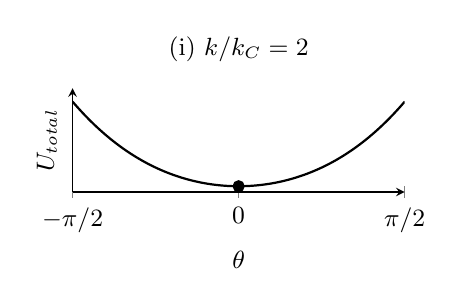
\begin{tikzpicture}
\begin{axis}[width=5.8cm,height=2.9cm,axis lines=left,
title={(i) $k/k_C=2$},title style={font=\small},
xmin=-90,xmax=90,ymin=0.9,ymax=2.7,
xtick={-90,0,90},xticklabels={$-\pi/2$,$0$,$\pi/2$},ytick=\empty,
xlabel={$\theta$},ylabel={$U_{total}$},label style={font=\small},tick label style={font=\small}]
\addplot[thick,domain=-90:90,samples=121]{cos(x)+1.0*(x*pi/180)^2};
\addplot[only marks,mark=*]coordinates{(0,1)};
\end{axis}
\end{tikzpicture}
\end{minipage}\hfill
\begin{minipage}{0.48\linewidth}
\centering
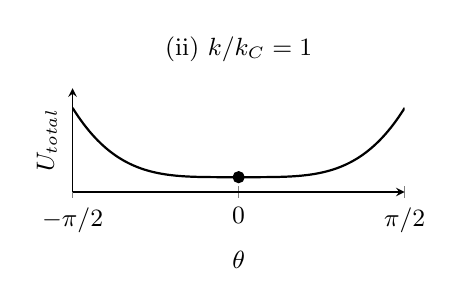
\begin{tikzpicture}
\begin{axis}[width=5.8cm,height=2.9cm,axis lines=left,
title={(ii) $k/k_C=1$},title style={font=\small},
xmin=-90,xmax=90,ymin=0.95,ymax=1.3,
xtick={-90,0,90},xticklabels={$-\pi/2$,$0$,$\pi/2$},ytick=\empty,
xlabel={$\theta$},ylabel={$U_{total}$},label style={font=\small},tick label style={font=\small}]
\addplot[thick,domain=-90:90,samples=121]{cos(x)+0.5*(x*pi/180)^2};
\addplot[only marks,mark=*]coordinates{(0,1)};
\end{axis}
\end{tikzpicture}
\end{minipage}

\vspace{1mm}

\begin{minipage}{0.48\linewidth}
\centering
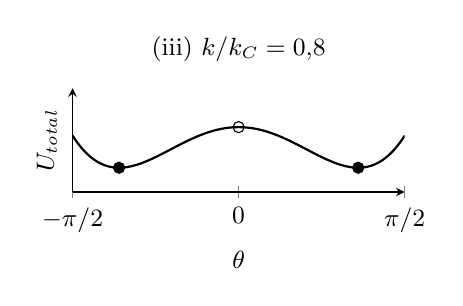
\begin{tikzpicture}
\begin{axis}[width=5.8cm,height=2.9cm,axis lines=left,
title={(iii) $k/k_C=0{,}8$},title style={font=\small},
xmin=-90,xmax=90,ymin=0.9,ymax=1.06,
xtick={-90,0,90},xticklabels={$-\pi/2$,$0$,$\pi/2$},ytick=\empty,
xlabel={$\theta$},ylabel={$U_{total}$},label style={font=\small},tick label style={font=\small}]
\addplot[thick,domain=-90:90,samples=121]{cos(x)+0.4*(x*pi/180)^2};
\addplot[only marks,mark=o]coordinates{(0,1)};
\addplot[only marks,mark=*]coordinates{(-64.8,0.9374) (64.8,0.9374)};
\end{axis}
\end{tikzpicture}
\end{minipage}\hfill
\begin{minipage}{0.48\linewidth}
\centering
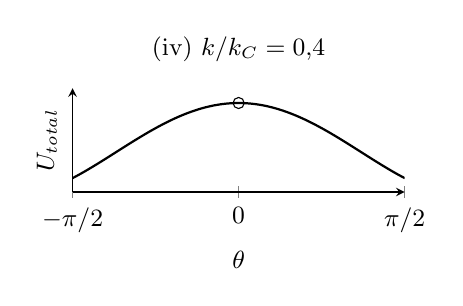
\begin{tikzpicture}
\begin{axis}[width=5.8cm,height=2.9cm,axis lines=left,
title={(iv) $k/k_C=0{,}4$},title style={font=\small},
xmin=-90,xmax=90,ymin=0.4,ymax=1.1,
xtick={-90,0,90},xticklabels={$-\pi/2$,$0$,$\pi/2$},ytick=\empty,
xlabel={$\theta$},ylabel={$U_{total}$},label style={font=\small},tick label style={font=\small}]
\addplot[thick,domain=-90:90,samples=121]{cos(x)+0.2*(x*pi/180)^2};
\addplot[only marks,mark=o]coordinates{(0,1)};
\end{axis}
\end{tikzpicture}
\end{minipage}
\end{center}

\noindent\emph{Esboços qualitativos (escala vertical independente em cada painel). Cheio: estável (mínimo); vazado: instável (máximo).}

ANSWER: (a) $k_C=\dfrac{MgL}{2}$; (b) $k/k_C>1$ ou $k/k_C=1$: um equilíbrio, $\theta=0$, estável (no caso $k/k_C=1$, degenerado); $\frac{2}{\pi}<k/k_C<1$: três equilíbrios, com $\theta=0$ instável e $\pm\theta_e$ estáveis, onde $\frac{\operatorname{sen}\theta_e}{\theta_e}=\frac{k}{k_C}$; $0<k/k_C\le\frac{2}{\pi}$: somente $\theta=0$ no intervalo, instável; (c) poço único ($k/k_C>1$), poço quártico ($k/k_C=1$), duplo poço com máximo local em $\theta=0$ e mínimos em $\pm\theta_e$ ($\frac{2}{\pi}<k/k_C<1$; para $k/k_C>\frac{8}{\pi^2}$, $\theta=0$ é só máximo local), e máximo monotônico decrescente ($0<k/k_C\le\frac{2}{\pi}$).%
\newpage%
\section*{Questão 2}

\section*{Solução}

\textbf{Hipóteses e referencial.} Massa tratada como ponto material, de modo que o choque não induz rotação (o impulso do solo passa pelo centro de massa). Resistência do ar desprezada; $g$ constante; solo horizontal, fixo e liso, em $y=0$, com a origem $O$ sobre ele; $x$ horizontal e $y$ vertical; energia potencial gravitacional referida ao solo; choques instantâneos; coeficiente de restituição $e=0{,}7$ em todos os choques. Como o solo está em repouso, a restituição de Newton para a componente normal é $|v'_y| = e\,|v_y|$, com inversão do sentido.

\textbf{1) Velocidade inicial.}
\begin{align*}
v_{x0} &= V\cos 30^\circ = \frac{\sqrt{3}}{2}V, & v_{y0} &= V\operatorname{sen}30^\circ = \frac{V}{2}.
\end{align*}

\textbf{2) Componente horizontal.} No voo, a única força é o peso, que é vertical. No choque, o solo liso só pode exercer força normal, logo $\Delta p_x = 0$. Portanto $v_x = \frac{\sqrt{3}}{2}V$ é constante para todo $t$.

\textbf{3) Componente vertical.} Seja $u_k$ o módulo da velocidade vertical logo após o evento $k$, sendo $k=0$ o lançamento e $k\ge 1$ o $k$-ésimo choque. Tem-se $u_0 = V/2$. No voo, $a_y=-g$ e, pela conservação da energia mecânica (ou por Torricelli), ao voltar a $y=0$ a massa tem velocidade de módulo $u_k$ dirigida para baixo. Esse é o módulo da velocidade de impacto do choque seguinte. Pela restituição, a velocidade após esse choque é $u_{k+1} = e\,u_k$. Por indução,
\begin{align*}
u_n = e^{n}\,u_0 = e^{n}\frac{V}{2}.
\end{align*}

\textbf{4) Item a: altura máxima após $n$ choques.} Após o $n$-ésimo choque, a massa sobe até o ápice, onde $v_y=0$. Por Torricelli, com aceleração $-g$ e $y=0$ no choque,
\begin{align*}
0 = u_n^2 - 2gH_n \quad\Rightarrow\quad H_n = \frac{u_n^2}{2g} = \frac{e^{2n}V^2}{8g} = \frac{(0{,}49)^{n}\,V^2}{8g}.
\end{align*}
Equivalentemente, $H_n = \dfrac{e^{2n}V^2\operatorname{sen}^2 30^\circ}{2g}$. A altura depende de $e^2$, pois a restituição reduz a velocidade vertical por $e$ e, portanto, a energia cinética vertical por $e^2$. A componente horizontal não interfere, já que $y$ depende apenas de $v_y$. Para $n=0$, $H_0 = V^2/(8g)$ é a altura do primeiro arco. Como os arcos decrescem monotonicamente, $H_n$ também é a altura máxima de todo o movimento posterior ao $n$-ésimo choque.

\textbf{5) Energia mecânica.} Tome $E = \frac{1}{2}m\left(v_x^2+v_y^2\right)+mgy$. Durante o voo, $E$ se conserva, pois só atua o peso. No $n$-ésimo choque, somente $v_y$ muda: a energia cinética vertical passa de $\frac{1}{2}m\,u_{n-1}^2$ para $\frac{1}{2}m\,e^2u_{n-1}^2$. A perda $\frac{1}{2}m(1-e^2)u_{n-1}^2$ é positiva, de modo que $E$ decresce em degraus. Imediatamente após o $n$-ésimo choque ($y=0$),
\begin{align*}
E_n = \frac{m}{2}\left(\frac{3}{4}V^2 + \frac{e^{2n}V^2}{4}\right) = \frac{mV^2}{8}\left(3+e^{2n}\right).
\end{align*}
Verificação: $E_0 = \frac{1}{2}mV^2$.

Por que a energia total: a potencial $mgy$ é nula no lançamento e em cada choque, logo seu mínimo se repete sem definir um instante próprio. A cinética atinge $\frac{3}{8}mV^2$ em cada ápice ($v_y=0$), também de forma recorrente. Só a energia total decresce monotonicamente e se estabiliza.

Como $e^{2n}>0$ para todo $n$ finito, $E_n > E_{\min}$ sempre, e
\begin{align*}
\lim_{n\to\infty}E_n = E_{\min} = \frac{3}{8}mV^2 = \frac{3}{4}E_0 = E_0\cos^2 30^\circ.
\end{align*}
Esse valor é a energia cinética horizontal, que não se dissipa no solo liso. O mínimo é atingido no instante limite $t_\infty$, ponto de acumulação dos choques, que ocorre em tempo finito. Para $t\ge t_\infty$ a componente vertical está nula, a massa desliza sobre o solo liso com $v_x$ constante e $E = \frac{3}{8}mV^2$ se mantém.

\textbf{6) Item b: intervalo de tempo.} Cada arco é parabólico e simétrico: a subida e a descida duram $u_k/g$ cada. O arco que começa no evento $k$ dura
\begin{align*}
\tau_k = \frac{2u_k}{g} = \frac{2}{g}\,e^{k}\frac{V}{2} = e^{k}\frac{V}{g}.
\end{align*}
O $n$-ésimo choque ocorre em
\begin{align*}
t_n = \sum_{k=0}^{n-1}\tau_k = \frac{V}{g}\,\frac{1-e^{n}}{1-e},
\end{align*}
com $t_1 = V/g$, que é o primeiro voo. Como $0<e<1$, a série geométrica converge e o mínimo de energia é atingido em
\begin{align*}
\Delta t = t_\infty = \frac{V}{g}\sum_{k=0}^{\infty}e^{k} = \frac{V}{g(1-e)} = \frac{V}{0{,}3\,g} = \frac{10}{3}\,\frac{V}{g}\approx 3{,}33\,\frac{V}{g}.
\end{align*}
A massa $m$ não aparece em $\Delta t$: a aceleração vertical é $-g$ para qualquer $m$, e $e$ é adimensional.

\textbf{7) Verificações.}
\begin{itemize}
\item Unidades: $[H_n] = \dfrac{(\mathrm{m/s})^2}{\mathrm{m/s^2}} = \mathrm{m}$, $[\Delta t] = \dfrac{\mathrm{m/s}}{\mathrm{m/s^2}} = \mathrm{s}$, $[E] = \mathrm{kg\,(m/s)^2} = \mathrm{J}$.
\item Casos particulares: para $e=1$, $H_n = V^2/(8g)$ e $E_n = \frac{1}{2}mV^2$ são constantes e $t_\infty\to\infty$, como em quicadas elásticas. Para $e=0$, $H_n=0$ para $n\ge 1$, $E_1 = E_{\min}$ e $\Delta t = V/g$, que é o primeiro pouso.
\item Monotonia: $H_n$ e $E_n$ decrescem com $n$, e $E_{\min}/E_0 = \cos^2 30^\circ = 3/4$ coincide com a fração horizontal da energia inicial.
\item Ordem de grandeza: com $V=10\,\mathrm{m/s}$ e $g=10\,\mathrm{m/s^2}$, tem-se $H_0 = 1{,}25\,\mathrm{m}$, $H_1 \approx 0{,}61\,\mathrm{m}$, $H_2 \approx 0{,}30\,\mathrm{m}$ e $\Delta t \approx 3{,}3\,\mathrm{s}$.
\end{itemize}

ANSWER: (a) $H_n = \dfrac{(0{,}49)^{n}\,V^2}{8g} = \dfrac{e^{2n}V^2\operatorname{sen}^2 30^\circ}{2g}$, com $e=0{,}7$ e $H_0 = \dfrac{V^2}{8g}$; (b) $\Delta t = \dfrac{V}{g(1-0{,}7)} = \dfrac{10\,V}{3\,g}\approx 3{,}33\,\dfrac{V}{g}$, instante em que a energia atinge o mínimo $E_{\min} = \dfrac{3}{8}mV^2$ (no limite de infinitos choques).%
\newpage%
\section*{Questão 3}

\section*{Solução}

\textbf{Hipóteses, referencial e interpretação.} Origem $O$ no solo, sobre o eixo do carrossel, com $z$ para cima; o carrossel está no plano $z=h$. A massa é tratada como partícula, o ar é desprezado e $\alpha>0$ é constante, no sentido da figura (o sentido oposto apenas troca o sinal de $x$ e não altera $d$ nem $t^\ast$). Assim $\omega(t)=\alpha t$ e a borda do disco percorre o ângulo $\psi(t)=\alpha t^2/2$. Em $t=0$ a massa está em repouso em $(0,R,h)$. Usamos $\hat e_r$ e $\hat e_\varphi$, versores radial e tangencial ao carrossel. Além do enunciado, adotamos:
\begin{itemize}
\item o coeficiente cinético massa–carrossel, $\mu_k$, não é dado; supomos $\mu_k<\mu_e$ (o usual). Se $\mu_k\ge\mu_e$, a massa não deixaria a borda, contrariando o enunciado. Os resultados de $d$ e de $t^\ast$ não dependem do valor de $\mu_k$;
\item o choque com o solo é sem quique ($e=0$), com atrito de Coulomb $\mu_cN$ atuando durante o choque (justificado no item b);
\item ``ponto de contato com o solo'' é o ponto do primeiro contato (queda); o deslizamento posterior não entra em $d$.
\end{itemize}

\textbf{1) Aderência ao carrossel ($0\le t\le t_1$).} No referencial do solo, o ponto do disco onde está a massa tem aceleração
\[
\vec a_D=\alpha R\,\hat e_\varphi-\omega^2R\,\hat e_r,\qquad |\vec a_D|=R\sqrt{\alpha^2+\omega^4}.
\]
Na vertical não há aceleração, logo $N=mg$. Na horizontal a única força é o atrito estático $\vec f$, e a segunda lei de Newton dá $\vec f=m\vec a_D$. Como $|\vec f|\le\mu_eN=\mu_emg$, a aderência exige $R\sqrt{\alpha^2+\omega^4}\le\mu_eg$. O deslizamento começa em $t_1$, quando a igualdade é atingida. Com $\omega_1=\alpha t_1$:
\[
\omega_1^4=\frac{\mu_e^2g^2-\alpha^2R^2}{R^2},\qquad t_1=\frac{\left(\mu_e^2g^2-\alpha^2R^2\right)^{1/4}}{\alpha\sqrt R},\qquad \omega_1^2R=\sqrt{\mu_e^2g^2-\alpha^2R^2},\qquad \omega_1R=\sqrt R\left(\mu_e^2g^2-\alpha^2R^2\right)^{1/4}.
\]
Essas expressões são reais para $\mu_eg>\alpha R$ (caso principal; o outro é tratado ao final).

\textbf{2) Abandono da borda ($t\ge t_1$).} Seja $\vec u=\vec v-\vec v_D$ a velocidade da massa relativa ao ponto do disco. Então $\dot{\vec u}=\vec a-\vec a_D$, com $m\vec a=\vec f_c$ e, pelo atrito cinético, $\vec f_c=-\mu_kmg\,\hat u$. Em $t_1^+$ temos $\vec u=0$, e a direção de $\vec u$ decorre da própria dinâmica. Testemos $\vec f_c=\mu_kmg\,\hat a_D$. Então
\[
\dot{\vec u}=\left(\mu_kg-|\vec a_D|\right)\hat a_D .
\]
Como $|\vec a_D|\ge\mu_eg>\mu_kg$, $\dot{\vec u}$ aponta para $-\hat a_D$. Logo $\vec u$ cresce nesse sentido, e o atrito, oposto a $\vec u$, é de fato $+\mu_kmg\,\hat a_D$: a hipótese é autoconsistente. Assim o atrito não é tangencial. Em $t_1$ temos $|\vec a_D|=\mu_eg$ e $\hat a_D\cdot\hat e_r=-\omega_1^2R/(\mu_eg)$, de modo que a componente radial do atrito é
\[
f_r=-\frac{\mu_k}{\mu_e}\,m\,\omega_1^2R .
\]
Em coordenadas polares inerciais, $m(\ddot r-r\dot\varphi^2)=f_r$, pois a normal é vertical. Em $t_1$ temos $r=R$, $\dot r=0$ e $\dot\varphi=\omega_1$, logo
\[
\ddot r=\omega_1^2R\left(1-\frac{\mu_k}{\mu_e}\right)>0 .
\]
A massa passa a ter $r>R$, sai do disco e perde o contato com o carrossel. Em $t_1$ a velocidade relativa é nula, então a velocidade de abandono é tangencial: $\vec v_0=\omega_1R\,\hat e_\varphi$, horizontal, com $v_0=\omega_1R$.

\textbf{Queda livre.} Fora do disco não há força horizontal (ar desprezado), logo $v_x=v_0$ é constante. A queda de altura $h$, partindo de velocidade vertical nula, dá
\[
t_q=\sqrt{\frac{2h}{g}},\qquad v_z=gt_q=\sqrt{2gh}.
\]

\textbf{a)} O abandono ocorre no ponto $R\,\hat e_r$ (projeção no plano $xy$), e $\vec v_0\perp\hat e_r$. Durante $t_q$ a massa se desloca $v_0t_q$ na direção $\hat e_\varphi$. Logo $\vec{OP}=R\,\hat e_r+v_0t_q\,\hat e_\varphi$, onde $P$ é o ponto de contato com o solo, e por Pitágoras
\[
d=\sqrt{R^2+(v_0t_q)^2},\qquad (v_0t_q)^2=\omega_1^2R^2\,\frac{2h}{g}=\frac{2hR}{g}\sqrt{\mu_e^2g^2-\alpha^2R^2},
\]
pois $\omega_1^2R^2=R\,\omega_1^2R$. Portanto
\[
d=\sqrt{R^2+\frac{2hR}{g}\sqrt{\mu_e^2g^2-\alpha^2R^2}} .
\]

\textbf{b)} Impacto. Em $t_1+t_q$ a massa atinge o solo com velocidade $(v_0,0,-v_z)$. Sem quique, $e=0$: a componente vertical se anula e o impulso normal é $J_N=mv_z$ (a normal é impulsiva; peso e forças finitas são desprezíveis no choque). Enquanto desliza, o atrito é $f=\mu_cN(t)$, oposto à velocidade horizontal. Como $N$ é impulsivo, o impulso do atrito é $\int\mu_cN\,dt=\mu_cmv_z$, da mesma ordem do impulso normal, e portanto não é desprezível. Desprezá-lo equivaleria a atrito nulo durante o choque, o que contradiz o deslizamento. Após o choque, $N=mg$ e a desaceleração é $\mu_cg$.

Teorema do impulso na horizontal, de logo antes do impacto (momento $mv_0$, pois no voo não há força horizontal) até a parada, com $t_s$ o tempo de deslizamento após o choque:
\[
0-mv_0=-\mu_cmv_z-\mu_cmg\,t_s\quad\Rightarrow\quad t_s=\frac{v_0}{\mu_cg}-\frac{v_z}{g}=\frac{\omega_1R}{\mu_cg}-t_q .
\]
Isso vale se $t_s>0$, isto é, $\omega_1R>\mu_c\sqrt{2gh}$, condição de que o deslizamento persista durante todo o choque. O instante de parada é $t^\ast=t_1+t_q+t_s$, e o tempo de queda se cancela:
\[
t^\ast=t_1+\frac{\omega_1R}{\mu_cg}.
\]
Se $\omega_1R\le\mu_c\sqrt{2gh}$, o impulso de atrito no choque anula a velocidade horizontal ($\mu_cmv_z\ge mv_0$) e a massa para no impacto: $t^\ast=t_1+t_q$. Os dois casos se resumem a $t^\ast=t_1+\max\left\{\sqrt{2h/g},\ \omega_1R/(\mu_cg)\right\}$, contínua em $\omega_1R=\mu_c\sqrt{2gh}$.

Substituindo $t_1$ e $\omega_1R$:
\[
t^\ast=\frac{\left(\mu_e^2g^2-\alpha^2R^2\right)^{1/4}}{\alpha\sqrt R}+\frac{\sqrt R\left(\mu_e^2g^2-\alpha^2R^2\right)^{1/4}}{\mu_cg}=\frac{\left(\mu_e^2g^2-\alpha^2R^2\right)^{1/4}\left(\mu_cg+\alpha R\right)}{\alpha\,\mu_c\,g\,\sqrt R}.
\]

\textbf{Modelagem do choque.} O resultado usa o atrito de Coulomb durante o choque, que é a lei de atrito dada ($f=\mu_cN$) aplicada ao impulso normal. A leitura alternativa, que despreza o impulso de atrito no choque, daria $t'=t^\ast+\sqrt{2h/g}$. Essa leitura só seria boa se $\mu_cv_z\ll v_0$; no exemplo abaixo o impulso de atrito é $\mu_cv_z\approx0{,}35\,v_0$, então a diferença é grande.

\textbf{Caso $\mu_eg\le\alpha R$.} Em $t=0^+$ o atrito estático não basta. Enquanto desliza, a massa recebe aceleração horizontal de módulo $\mu_kg<\mu_eg\le\alpha R$, com atrito cinético tangencial para frente. A borda, por sua vez, acelera com $\alpha R$, de modo que a velocidade da massa ($\le\mu_kgt$) fica sempre abaixo da velocidade da borda ($\alpha Rt$). Em primeira ordem em $t$, a trajetória é a reta tangente ao rim no ponto de partida. A distância à origem é $\rho(t)=\sqrt{R^2+(\mu_kgt^2/2)^2}>R$ para todo $t>0$. Logo a massa sai da borda imediatamente, com velocidade $\mu_kgt\to0$. Então $d=R$, e sem velocidade horizontal no solo não há deslizamento: $t^\ast=\sqrt{2h/g}$. Este caso é o limite $\mu_eg\to\alpha R$ das fórmulas gerais, onde $t_1\to0$.

\textbf{Verificações.}
\begin{itemize}
\item Unidades: $(\mu_e^2g^2-\alpha^2R^2)^{1/4}$ tem unidade $\mathrm{m}^{1/2}\,\mathrm{s}^{-1}$ e $\alpha\sqrt R$ tem unidade $\mathrm{s}^{-2}\,\mathrm{m}^{1/2}$, logo $t_1$ está em s. O termo $\omega_1R/(\mu_cg)$ tem unidade $(\mathrm{m}/\mathrm{s})/(\mathrm{m}/\mathrm{s}^2)=\mathrm{s}$. Em $d$, $hR/g$ tem unidade $\mathrm{m}\cdot\mathrm{s}^2$ e $\sqrt{\mu_e^2g^2-\alpha^2R^2}$ tem unidade $\mathrm{m}/\mathrm{s}^2$, de modo que o radicando é $\mathrm{m}^2$ e $d$ está em m.
\item Limite $\alpha\to0$: $\omega_1^2R=\mu_eg$ e $d\to\sqrt{R^2+2\mu_ehR}$, como em rotação uniforme. Além disso $t_1\to\infty$: a massa acompanha o disco por um tempo arbitrariamente longo antes de deslizar.
\item Limite $h\to0$: $t_q\to0$ e $t^\ast=t_1+v_0/(\mu_cg)$, pois não há queda e a massa desliza diretamente.
\item Limite $\mu_eg\to\alpha R$: $t_1\to0$, $d\to R$ e $t^\ast\to\sqrt{2h/g}$, em continuidade com o caso $\mu_eg\le\alpha R$.
\item Exemplo numérico: $g=10$, $R=2$, $h=1{,}5$, $\alpha=0{,}5$, $\mu_e=0{,}5$, $\mu_c=0{,}2$ e, apenas para verificar $\mu_k<\mu_e$, $\mu_k=0{,}3$. Então $\mu_eg=5>\alpha R=1$, $\omega_1=6^{1/4}\approx1{,}565$ rad/s, $t_1\approx3{,}130$ s, $v_0=\omega_1R\approx3{,}130$ m/s, $t_q=\sqrt{0{,}3}\approx0{,}548$ s e $d\approx2{,}634$ m, da ordem de $R$. Como $\mu_c\sqrt{2gh}\approx1{,}095<v_0$, há deslizamento após o choque e $t^\ast\approx4{,}695$ s. Com o impulso de atrito no choque desprezado, $t'\approx5{,}243$ s. Em $t_1$, $\ddot r=\omega_1^2R(1-\mu_k/\mu_e)\approx1{,}96$ m/s$^2>0$, o que confirma o abandono.
\end{itemize}

ANSWER: a) $d=\sqrt{R^2+\dfrac{2hR}{g}\sqrt{\mu_e^2g^2-\alpha^2R^2}}$ (para $\mu_eg>\alpha R$; se $\mu_eg\le\alpha R$, $d=R$); b) $t^\ast=t_1+\dfrac{\omega_1R}{\mu_cg}=\dfrac{\left(\mu_e^2g^2-\alpha^2R^2\right)^{1/4}\left(\mu_cg+\alpha R\right)}{\alpha\,\mu_c\,g\,\sqrt R}$ (para $\omega_1R>\mu_c\sqrt{2gh}$; caso contrário $t^\ast=t_1+\sqrt{2h/g}$; se $\mu_eg\le\alpha R$, $t^\ast=\sqrt{2h/g}$)%
\newpage%
\section*{Questão 4}

\section*{Solução}

\textbf{Hipóteses e dados.} O gás é ideal e monoatômico: $C_V=\frac{3}{2}R$ por mol, $U=\frac{3}{2}nRT=\frac{3}{2}PV$ e $\gamma=\frac{C_P}{C_V}=\frac{5}{3}$. As paredes e o pistão são adiabáticos ($Q=0$), o pistão não tem atrito, o recipiente de areia tem massa desprezível e o vácuo acima do pistão significa pressão externa nula. No equilíbrio inicial, o pistão (com a areia) dá
\[
P_iA=(m+M)g \quad\Rightarrow\quad P_i=\frac{(m+M)g}{A},\qquad V_i=Ah_i .
\]

\textbf{Item a.} A areia sai em processo quase estático: em cada instante o pistão está em equilíbrio mecânico, $PA=(m+M')g$, com $M'$ a areia restante. Como as paredes e o pistão são adiabáticos, o processo é adiabático e reversível, logo $PV^{\gamma}=\text{cte}$, com $\gamma=\frac{5}{3}$.

No estado final resta só o pistão: $P_f=\frac{mg}{A}$ e $V_f=Ah_f$. Então
\[
P_i(Ah_i)^{5/3}=P_f(Ah_f)^{5/3}\quad\Rightarrow\quad \left(\frac{h_f}{h_i}\right)^{5/3}=\frac{P_i}{P_f}=\frac{m+M}{m},
\]
\[
\boxed{h_f=h_i\left(\frac{m+M}{m}\right)^{3/5}}
\]
A área $A$, $n$ e $R$ não aparecem no resultado.

\textit{Verificações.} (i) Para $M\to 0$, $h_f\to h_i$. (ii) $h_f>h_i$, como esperado, pois o gás se expande ao perder peso. (iii) $\frac{T_f}{T_i}=\frac{P_fV_f}{P_iV_i}=\left(\frac{m}{m+M}\right)^{2/5}<1$: a expansão adiabática resfria o gás. (iv) Com $Q=0$, a primeira lei dá $W_{\text{gás}}=\int_{h_i}^{h_f}PA\,dh=\frac{3}{2}\left[(m+M)gh_i-mgh_f\right]=-\Delta U$, que é o resultado esperado.

\textbf{Item b.} Com a retirada instantânea, a força resultante inicial sobre o pistão é $PA-mg=Mg$, para cima. O pistão sobe, ultrapassa a posição de equilíbrio $h_f$, para momentaneamente em $h_{\max}$ e retorna. Sem dissipação, ele oscila entre $h_i$ e $h_{\max}$, e $h_{\max}$ é a primeira inversão do sentido do movimento.

Hipótese: as velocidades do pistão são da ordem de metros por segundo, muito menores que a velocidade do som no gás (centenas de metros por segundo). Assim a pressão é uniforme no gás em cada instante, a evolução é reversível e adiabática, e vale $PV^{5/3}=\text{cte}$ durante todo o movimento. Em particular, $P_{\max}=P_i\left(\frac{h_i}{h_{\max}}\right)^{5/3}$.

\textit{Passo 1 (teorema da energia cinética no pistão).} Entre o repouso em $h_i$ e o repouso em $h_{\max}$, $\Delta K=0$. As forças que realizam trabalho são o gás e o peso: $W_{\text{gás}}-mg(h_{\max}-h_i)=0$, logo
\[
W_{\text{gás}}=mg\,(h_{\max}-h_i).
\]

\textit{Passo 2 (primeira lei no gás).} Como $Q=0$,
\[
\Delta U_{\text{gás}}=-W_{\text{gás}}=-mg\,(h_{\max}-h_i).
\]

\textit{Passo 3 (variação da energia interna).} Com $U=\frac{3}{2}PV$, $AP_i=(m+M)g$ e $P_{\max}=P_i\left(\frac{h_i}{h_{\max}}\right)^{5/3}$:
\[
\Delta U=\frac{3}{2}A\left(P_{\max}h_{\max}-P_ih_i\right)=\frac{3}{2}(m+M)g\left[h_i^{5/3}h_{\max}^{-2/3}-h_i\right].
\]

\textit{Passo 4 (igualdade dos dois resultados).} Igualando e dividindo por $g$:
\[
\frac{3}{2}(m+M)\left[h_i^{5/3}h_{\max}^{-2/3}-h_i\right]=-m\,(h_{\max}-h_i),
\]
que se reescreve como
\[
\boxed{\,m\,(h_{\max}-h_i)=\frac{3}{2}(m+M)\,h_i\left[1-\left(\frac{h_i}{h_{\max}}\right)^{2/3}\right]\,}
\]

Essa equação é equivalente à conservação da energia $\frac{1}{2}mv^2+mgh+\frac{3}{2}PAh=\text{cte}$, pois $\frac{d}{dh}\left(\frac{3}{2}PAh\right)=-PA$. Com $y=(h_{\max}/h_i)^{1/3}$, ela vira $2m\,y^2(y^2+y+1)=3(m+M)(y+1)$, com $y\neq 1$.

\textit{Discussão da raiz.} Seja $x=h_{\max}/h_i$ e $F(x)=m(x-1)-\frac{3}{2}(m+M)\left(1-x^{-2/3}\right)$. Então $F(1)=0$ (raiz trivial, sem movimento) e $F'(x)=m-(m+M)x^{-5/3}$, que é negativa para $x$ entre 1 e $h_f/h_i$ e positiva depois. Como $F\to+\infty$, existe uma única raiz $x>1$, e ela satisfaz $h_{\max}>h_f$.

\textit{Limites.} Para $M\to 0$, $F'(x)=m(1-x^{-5/3})>0$ para $x>1$, então não há movimento, consistente com $h_f=h_i$. Para $M\ll m$, linearizando em torno de $h_i$ obtém-se $h_{\max}-h_i\approx\frac{6M}{5(m+M)}h_i\approx 2(h_f-h_i)$, como num oscilador simétrico em torno de $h_f$.

\textit{Exemplo numérico.} Para $m=2\,\text{kg}$, $M=3\,\text{kg}$ e $h_i=0,5\,\text{m}$: $h_f\approx 0,87\,\text{m}$ e, resolvendo a equação, $h_{\max}\approx 1,46\,\text{m}$. O movimento é assimétrico ($h_{\max}-h_f\approx 0,59\,\text{m}$ e $h_f-h_i\approx 0,37\,\text{m}$), então em geral $h_{\max}\neq 2h_f-h_i$.

ANSWER: (a) $h_f=h_i\left(\frac{m+M}{m}\right)^{3/5}$; (b) $m\,(h_{\max}-h_i)=\frac{3}{2}(m+M)\,h_i\left[1-\left(\frac{h_i}{h_{\max}}\right)^{2/3}\right]$, cuja raiz não trivial é única e satisfaz $h_{\max}>h_f$.%
\newpage%
\section*{Questão 5}

\section*{Solução}

\textbf{Hipóteses e convenções.}
\begin{itemize}
\item Paraxial: raios próximos ao eixo, $\sin\theta\approx\tan\theta\approx\theta$, e lei de Snell $n_1 i=n_2 r$, com $i$ e $r$ medidos a partir da normal. Vale $\lambda\ll p\ll D$ (óptica geométrica), $h\ll p$ e $h\ll D$.
\item Coordenadas: origem no vértice, $x$ no sentido da luz, $y$ para cima. Pela figura, $C=(-R,0)$ está do lado de $n_1$; a superfície é $(x+R)^2+y^2=R^2$ e as fontes são $S_\pm=(-p,\pm h)$.
\item Sinal de $R$: o centro está do lado incidente, logo $R_G=-R$ na convenção de dioptro, e a potência $(n_2-n_1)/R_G=-(n_2-n_1)/R$ é negativa. A superfície é divergente. Usar $+R$ trocaria o sinal de todos os resultados.
\item Fontes coerentes, em fase (fase inicial nula) e com amplitudes iguais por simetria. A fase nula é a condição para o ponto central estar sobre o eixo; é hipótese explícita.
\item O enunciado não diz em qual meio $\lambda$ é medido. Dou o resultado com $\lambda_0$ (vácuo) e com $\lambda_1=\lambda_0/n_1$ (meio das fontes). As duas formas são equivalentes.
\end{itemize}

\textbf{a) Posição horizontal da imagem.} Seja $Q=(x_Q,y_Q)$ o ponto em que o raio que sai de $(-p,0)$ atinge a superfície. Como $x_Q=-R+\sqrt{R^2-y_Q^2}\approx -y_Q^2/(2R)$ é de segunda ordem, $Q\approx(0,y_Q)$. Com as inclinações paraxiais:
\begin{itemize}
\item raio incidente: $\alpha_i=y_Q/p$;
\item normal, na direção de $\overrightarrow{CQ}\approx(R,y_Q)$: $\alpha_N=y_Q/R$;
\item raio refratado, que cruza o eixo em $(p',0)$: $\alpha_r=-y_Q/p'$.
\end{itemize}
Logo, medidos no mesmo sentido, $i=\alpha_i-\alpha_N=y_Q\left(\dfrac1p-\dfrac1R\right)$ e $r=\alpha_r-\alpha_N=-y_Q\left(\dfrac1{p'}+\dfrac1R\right)$. Pela lei de Snell, $n_1 i=n_2 r$. Dividindo por $y_Q\neq0$:
\[
\frac{n_1}{p}+\frac{n_2}{p'}=\frac{n_1-n_2}{R}
\qquad\Rightarrow\qquad
p'=-\frac{n_2\,R\,p}{n_1R+(n_2-n_1)\,p}.
\]
Como $n_2>n_1$ e $R,p>0$, o denominador é positivo e $p'<0$. A imagem é virtual, do lado de $n_1$ (mesmo lado das fontes), à distância $|p'|$ da interface.

Checagens: para $n_1=n_2$, $p'=-p$ (sem interface). Para $R\to\infty$, $p'=-n_2p/n_1$ (dioptro plano; a imagem fica mais afastada por $n_2/n_1$). Para $p\to\infty$, $p'\to -n_2R/(n_2-n_1)$, a posição do foco-imagem virtual do dioptro divergente. Exemplo: $n_1=1$, $n_2=1{,}5$, $R=10\,\mathrm{cm}$ e $p=5\,\mathrm{cm}$ dão $p'=-6\,\mathrm{cm}$, e $\dfrac15+\dfrac{1{,}5}{-6}=-0{,}05=\dfrac{1-1{,}5}{10}$.

\textbf{Posições verticais.} O raio de $S_+$ que passa por $C$ incide normalmente (a normal passa por $C$) e não se desvia. Sua reta é $SC$: $y=\dfrac{h\,(x+R)}{R-p}$. Pelo estigmatismo paraxial, os prolongamentos dos raios refratados de $S_+$ concorrem em $S'_+$, e este raio é um deles. Logo $S'_+$ está nessa reta, em $x=p'$:
\[
y'_+=\frac{h\,(p'+R)}{R-p}.
\]
Como $p'+R=\dfrac{n_1R\,(R-p)}{n_1R+(n_2-n_1)\,p}$, obtém-se
\[
y'_+=m\,h,\qquad m=\frac{n_1R}{n_1R+(n_2-n_1)\,p}.
\]
Pela simetria em relação ao eixo, $y'_-=-m\,h$. Assim,
\[
y'_\pm=\pm\frac{n_1R}{n_1R+(n_2-n_1)\,p}\,h.
\]
O fator $m$ depende só de $n_1$, $n_2$, $R$ e $p$; $h$ é a posição dada das fontes. Conferência: $m=-n_1p'/(n_2p)$, que é o aumento transversal da equação do dioptro. Como $m>0$, a imagem é direta. Para $R\to\infty$, $m=1$. No exemplo, $m=0{,}8$.

\textbf{b) Franja luminosa para $R\to\infty$.} A interface é plana. Calculo a diferença de caminho óptico diretamente, pelo princípio de Fermat. Seja $S=(-p,y_S)$ uma fonte, $P=(D,y)$ um ponto da tela e $Q=(0,u)$ o ponto de incidência na interface. Com $\sqrt{a^2+s^2}\approx a+\dfrac{s^2}{2a}$ para $s\ll a$:
\[
F(u)=n_1\sqrt{p^2+(u-y_S)^2}+n_2\sqrt{D^2+(y-u)^2}\approx n_1p+n_2D+\frac{A}{2}(u-y_S)^2+\frac{B}{2}(y-u)^2,
\]
com $A=n_1/p$ e $B=n_2/D$. O raio real é estacionário em $u$, ou seja, $A(u-y_S)=B(y-u)$. Então $u-y_S=\dfrac{B(y-y_S)}{A+B}$ e $y-u=\dfrac{A(y-y_S)}{A+B}$, e
\[
\mathrm{OPL}(S\to P)=n_1p+n_2D+\frac{AB}{2(A+B)}(y-y_S)^2=n_1p+n_2D+\frac{n_1n_2\,(y-y_S)^2}{2\,(n_1D+n_2p)},
\]
pois $\dfrac{AB}{A+B}=\dfrac{n_1n_2}{n_1D+n_2p}$. Conferência: para $n_1=n_2=n$, o último termo é $n(y-y_S)^2/[2(D+p)]$, a expansão do caminho reto $n\sqrt{(D+p)^2+(y-y_S)^2}$.

Para $y_S=\pm h$:
\[
\Delta\mathrm{OPL}=\mathrm{OPL}(S_-\to P)-\mathrm{OPL}(S_+\to P)=\frac{n_1n_2\left[(y+h)^2-(y-h)^2\right]}{2(n_1D+n_2p)}=\frac{2\,n_1n_2\,h\,y}{n_1D+n_2p}.
\]
As fontes são coerentes e em fase, e a diferença de fase em $P$ é $\Delta\varphi=k_0\,\Delta\mathrm{OPL}$, com $k_0=2\pi/\lambda_0$, constante no tempo. Com amplitudes iguais, $I\propto\cos^2(\Delta\varphi/2)$. Há máximos quando $\Delta\mathrm{OPL}=m\lambda_0$, com $m\in\mathbb{Z}$:
\[
y_m=\frac{m\,\lambda_0\,(n_1D+n_2p)}{2\,n_1n_2\,h}.
\]
O máximo central é $m=0$, em $y=0$. A primeira franja luminosa é $m=\pm1$, à distância
\[
y_1=\frac{\lambda_0\,(n_1D+n_2p)}{2\,n_1n_2\,h}.
\]
Interpretação: com $L=D+\dfrac{n_2p}{n_1}=\dfrac{n_1D+n_2p}{n_1}$, a distância das imagens $(-n_2p/n_1,\pm h)$ à tela, tem-se $y_1=\dfrac{\lambda_2L}{2h}$, com $\lambda_2=\lambda_0/n_2$. É a fenda dupla de Young com fontes virtuais separadas por $2h$.

Como $p\ll D$, $L\approx D$ e $y_1\approx\dfrac{\lambda_0D}{2n_2h}$. A correção relativa é $n_2p/(n_1D)$, que vale $1{,}5\%$ para $n_2/n_1=1{,}5$ e $p/D=0{,}01$. Validade: $y_1\ll L$ exige $\lambda_2\ll 2h$, e $h\ll p$ mantém as fontes paraxiais.

Exemplo: $\lambda_0=500\,\mathrm{nm}$, $n_1=1$, $n_2=1{,}5$, $p=1\,\mathrm{cm}$, $D=1\,\mathrm{m}$ e $h=0{,}1\,\mathrm{mm}$, com $h\ll p\ll D$ e $\lambda\ll p$. Então $\lambda_2\approx333\,\mathrm{nm}$, $L=1{,}015\,\mathrm{m}$, $y_1\approx1{,}69\,\mathrm{mm}$ pela fórmula completa e $1{,}67\,\mathrm{mm}$ pela aproximada. Além disso, $\lambda_2/(2h)\approx1{,}7\times10^{-3}\ll1$.

Verificações: $\lambda_0D/(n_2h)$ tem unidade de metro. Sem interface ($n_1=n_2=n$), $y_1=\lambda_n(D+p)/(2h)$, o resultado de Young com a tela a $D+p$ das fontes. Com $\lambda_1=\lambda_0/n_1$, $y_1=\dfrac{\lambda_1(n_1D+n_2p)}{2n_2h}\approx\dfrac{n_1\lambda_1D}{2n_2h}$.

ANSWER: a) $p'=-\dfrac{n_2Rp}{n_1R+(n_2-n_1)p}$ (imagem virtual, do lado de $n_1$); posições verticais $y'_\pm=\pm\dfrac{n_1R}{n_1R+(n_2-n_1)p}\,h$ (imagem direta). b) $y_1=\dfrac{\lambda_0(n_1D+n_2p)}{2n_1n_2h}\approx\dfrac{\lambda_0D}{2n_2h}$, com $\lambda_0$ o comprimento de onda no vácuo; equivalentemente, $y_1=\dfrac{\lambda_1(n_1D+n_2p)}{2n_2h}\approx\dfrac{n_1\lambda_1D}{2n_2h}$, com $\lambda_1=\lambda_0/n_1$ o comprimento de onda no meio das fontes.%
\newpage%
\section*{Questão 6}

\section*{Solução}

\textbf{Modelo e hipóteses.} Pela figura, as placas são verticais e a mola é horizontal, normal às placas. Além do enunciado, adoto as hipóteses usuais de modelagem: (i) fios flexíveis, de massa desprezível, que apenas conduzem carga e não exercem força horizontal; o peso das placas é paralelo a elas e é sustentado pelos fios, logo não entra no balanço normal; (ii) mola ideal de massa desprezível, com $F=k\Delta$ para compressão $\Delta$ (linearidade); (iii) chaves, fonte, fios e voltímetro ideais, sem dissipação elétrica (o voltímetro não drena carga). Como $d\ll a$, cada placa é um plano infinito, com campo uniforme entre elas e sem efeito de borda; a capacitância das placas com separação $x$ é $C_p(x)=\varepsilon_0A/x$. Por hipótese, $C_p(d)=C$, logo $\varepsilon_0A=Cd$. Em $t_3$ o enunciado afirma equilíbrio: usamos conservação de carga e equilíbrio de forças, sem resolver o transitório.

\textbf{Estado em $t_2$.} Com $S_1$ fechada até a carga completa, a corrente é nula, não há queda em $R$ e $V_C=\varepsilon$; a armadura superior de $C$ tem carga $C\varepsilon$. Ao abrir $S_1$, o ramo $R$–$\varepsilon$ deixa de pertencer ao circuito: não há mais fonte nem resistor no caminho, portanto não se aplica $\tau=RC$ ao processo seguinte. As placas estão neutras, separadas por $d$, com a mola em seu comprimento natural (força nula). O voltímetro lê $V(t_2)=\varepsilon$.

\textbf{Passo 1: conservação de carga e $V(x)$.} Ao fechar $S_2$, a armadura superior de $C$ e a placa 1 formam um nó isolado: fios, voltímetro e chaves ideais, e nenhuma fonte ligada. Sua carga total, $C\varepsilon$, se conserva. Seja $q$ a carga que passa de $C$ para a placa 1, que fica com $+q$; a placa 2 fica com $-q$, pois as placas são neutras no total. A armadura superior de $C$ fica com $C\varepsilon-q$. Como $C$ e as placas estão em paralelo entre os mesmos dois nós, ambos têm a mesma tensão $V$:

\[ V=\frac{C\varepsilon-q}{C}\qquad (1) \]

\[ V=\frac{q}{C_p(x)}=\frac{q\,x}{Cd}\qquad (2) \]

De (1), $q=C(\varepsilon-V)$; em (2), $Vd=(\varepsilon-V)x$. Assim

\[ V(x)=\frac{\varepsilon\,x}{x+d},\qquad q(x)=\frac{C\varepsilon\,d}{x+d}. \]

Como $dV/dx=\varepsilon d/(x+d)^2>0$, $V$ é biunívoca em $x$. Logo após fechar $S_2$ as placas ainda não se moveram ($x=d$), e $V=\varepsilon/2$ (dois capacitores iguais dividem a carga igualmente). Como $V(t_3)=\varepsilon/4<\varepsilon/2$, a separação diminuiu: $x_3<d$.

\textbf{Item a.} Em (1), com $V_3=\varepsilon/4$:

\[ \frac{\varepsilon}{4}=\frac{C\varepsilon-q_3}{C}\quad\Rightarrow\quad q_3=\frac{3}{4}\,C\varepsilon. \]

Essa é a carga que sai da armadura superior de $C$ e vai para a placa 1 (restam $C\varepsilon/4$ em $C$).

\textbf{Item b.} $V(x_3)=\varepsilon/4$ dá $4x_3=x_3+d$, logo $x_3=d/3$. Conferência: $C_p(x_3)=3C$ e $q_3=C_p V_3=3C\varepsilon/4$. Com comprimento natural $d$, a mola fica comprimida de

\[ \Delta=d-x_3=\frac{2}{3}\,d. \]

\textbf{Item c.} Cada placa tem densidade $\sigma=q/A$ e está no campo de plano infinito da outra, de módulo $\sigma/(2\varepsilon_0)$. A força atrativa sobre cada placa é

\[ F=\sigma\cdot\frac{\sigma}{2\varepsilon_0}\cdot A=\frac{q^2}{2\varepsilon_0A}=\frac{q^2}{2Cd}. \]

Em $t_3$: $F=\dfrac{(3C\varepsilon/4)^2}{2Cd}=\dfrac{9\,C\varepsilon^2}{32\,d}$.

Equilíbrio normal de cada placa: a mola ideal, de massa nula e comprimida, empurra cada placa para fora com $k\Delta$; a atração elétrica $F$ puxa cada placa para dentro. Logo $k\Delta=F$ (por placa, não $2F$):

\[ k=\frac{F}{\Delta}=\frac{9\,C\varepsilon^2}{32\,d}\cdot\frac{3}{2d}=\frac{27\,C\varepsilon^2}{64\,d^2}=\frac{27\,\varepsilon_0a^2\,\varepsilon^2}{64\,d^3}. \]

\textbf{Verificação da força pela energia.} Com a carga total $C\varepsilon$ conservada, a energia elétrica é $U_e=\dfrac{(C\varepsilon)^2}{2(C+C_p)}=\dfrac{C\varepsilon^2x}{2(x+d)}$. Então

\[ \frac{dU_e}{dx}=\frac{C\varepsilon^2d}{2(x+d)^2}=\frac{q(x)^2}{2\varepsilon_0A}=F(x). \]

A igualdade é um argumento de envelope: a carga se redistribui até $V_C=V_{\text{placas}}$, isto é, minimiza $W(q,x)=\dfrac{(C\varepsilon-q)^2}{2C}+\dfrac{q^2x}{2\varepsilon_0A}$ em $q$ (supondo redistribuição elétrica quase estática, sempre no mínimo). Então $dU_e/dx=\partial W/\partial x|_q=q^2/(2\varepsilon_0A)$.

\textbf{Estabilidade (breve).} Com $0<x$, a energia efetiva é $U(x)=U_e(x)+\frac{k}{2}(d-x)^2$, com

\[ U'(x)=\frac{C\varepsilon^2d}{2(x+d)^2}-k(d-x),\qquad U''(x)=k-\frac{C\varepsilon^2d}{(x+d)^3}. \]

O equilíbrio exige $k(d-x)(x+d)^2=C\varepsilon^2d/2$. A função $h(x)=(d-x)(x+d)^2$ tem $h'(x)=(x+d)(d-3x)$, com máximo em $x=d/3$, onde $h=32d^3/27$. Portanto há equilíbrio se, e somente se, $k\geq k_c=\dfrac{27\,C\varepsilon^2}{64\,d^2}$. O valor obtido é exatamente $k_c$, e então $U'=U''=0$ em $x=d/3$: o equilíbrio em $t_3$ é o limiar de estabilidade. Para $k>k_c$ há dois equilíbrios, sendo $x>d/3$ estável ($U''>0$) e $x<d/3$ instável; para $k<k_c$ não há equilíbrio e as placas colapsam. Em $k=k_c$, $U'\geq 0$ com zero único em $d/3$: na dinâmica conservativa, as placas passam por $d/3$ com velocidade não nula e colapsam; parar exatamente ali exige dissipação mecânica ajustada. Isso não altera os resultados de a), b) e c).

\textbf{Verificações.}
\begin{itemize}
\item Unidades: $q^2/(2Cd)$ tem unidade $\text{C}^2/(\text{F}\cdot\text{m})=\text{J}/\text{m}=\text{N}$; como $C\varepsilon^2$ é energia, $k$ está em $\text{J}/\text{m}^2=\text{N}/\text{m}$.
\item Sinais: $F$ é atrativa, $\Delta>0$ (compressão), e $x_3<d$ é compatível com $V(x)$ crescente.
\item Casos-limite: em $x=d$, $V=\varepsilon/2$ e $q=C\varepsilon/2$; em $x\to0$, $C_p\to\infty$, $V\to0$ e $q\to C\varepsilon$. Ambos satisfazem (1) e (2).
\item Aritmética exata com $C=\varepsilon=d=1$: $x=1/3$ dá $V=1/4$, $q=3/4$, $F=9/32$, $k=27/64$, $dU_e/dx=9/32$ e $U'=U''=0$.
\end{itemize}

ANSWER: a) $q=\frac{3}{4}\,C\varepsilon$; b) $\Delta=\frac{2}{3}\,d$ (compressão; placas a $d/3$); c) $k=\frac{27\,C\varepsilon^2}{64\,d^2}=\frac{27\,\varepsilon_0 a^2\,\varepsilon^2}{64\,d^3}$%
\newpage%
\section*{Questão 7}

\section*{Solução}

\textbf{Montagem e hipóteses.} Tome $V_C=0$. Na figura ampliada, o traço longo do símbolo da bateria (polo positivo, convenção usual) está no lado superior, ligado ao fio que chega a $A$; logo $V_A=V_s$. Trocar a polaridade apenas troca o sinal de $V_o$, sem alterar o módulo pedido em (a). Com fonte e voltímetro ideais, não há corrente na diagonal $DB$, e a ponte se reduz a dois divisores independentes, $ADC$ (braços $R_1$ e $R_3$) e $ABC$ (braços $R_2$ e $R_4$):
\[
V_D=V_s\,\frac{R_3}{R_1+R_3},\qquad V_B=V_s\,\frac{R_4}{R_2+R_4}.
\]
Escreva $R_i=R_0(1+x_i)$, com $x_i=G\varepsilon_i+\alpha\Delta T$ se o braço $i$ é extensômetro ($\varepsilon_i$ é a deformação do ponto de fixação) e $x_i=0$ se é resistor $R_0$. Com todos os $x_i=0$, $V_o=0$, como esperado para a ponte equilibrada.

\textbf{Linearização.} A expressão exata é
\[
V_o=V_s\left[\frac{1+x_3}{2+x_1+x_3}-\frac{1+x_4}{2+x_2+x_4}\right].
\]
Seja $y=(x_1+x_3)/2\ll 1$. Usando $(1+y)^{-1}\approx 1-y$ e descartando produtos de pequenas correções ($x_1x_3$, $x_3y$, etc.):
\[
\frac{1+x_3}{2(1+y)}\approx\frac{1+x_3}{2}\,(1-y)\approx\frac12+\frac{x_3-x_1}{4}.
\]
Analogamente, $\dfrac{1+x_4}{2+x_2+x_4}\approx\dfrac12+\dfrac{x_4-x_2}{4}$. Subtraindo,
\[
V_o\approx\frac{V_s}{4}\,(x_2+x_3-x_1-x_4)=\frac{V_s}{4}\sum_{i=1}^{4}\sigma_i\,x_i,
\]
com $\sigma_1=\sigma_4=-1$ e $\sigma_2=\sigma_3=+1$. As parcelas $V_s/2$ se cancelam, o que confirma a saída nula da ponte equilibrada. Braços opostos ($R_1$ com $R_4$, e $R_2$ com $R_3$) têm o mesmo sinal; braços adjacentes (que compartilham um vértice) têm sinais opostos.

\textbf{Item a.} Com um único extensômetro, $x_k=x=G\varepsilon+\alpha\Delta T$ e os demais $x_i=0$. Então $V_o=\pm\frac{V_s}{4}\,x$, com sinal negativo para $k=1$ ou $k=4$ e positivo para $k=2$ ou $k=3$. Conferência exata com o extensômetro em $R_1$: $V_D=\dfrac{V_s}{2+x}$ e $V_B=\dfrac{V_s}{2}$, logo
\[
V_o=\frac{V_s}{2+x}-\frac{V_s}{2}=-\frac{V_s\,x}{4}\cdot\frac{1}{1+x/2}\approx-\frac{V_s\,x}{4}\left(1-\frac{x}{2}\right)\approx-\frac{V_s\,x}{4},
\]
usando $(1+x/2)^{-1}\approx 1-x/2$ e descartando o termo em $x^2$. Portanto
\[
|V_o|=\frac{V_s}{4}\,\bigl|G\varepsilon+\alpha\Delta T\bigr|.
\]
Como $\varepsilon$ e $\Delta T$ entram somados, um único extensômetro não separa deformação de temperatura. Numericamente, com $V_s=10\,\mathrm{V}$, $G=2$ e $\varepsilon=10^{-4}$, tem-se $\dfrac{V_s}{4}=2{,}5\,\mathrm{V}$ e $G\varepsilon=2\cdot 10^{-4}$, logo $|V_o|=0{,}5\,\mathrm{mV}$. Um erro térmico $\alpha\Delta T=10^{-4}$ já produz $0{,}25\,\mathrm{mV}$, metade desse sinal.

\textbf{Item b.} Objetivos: (i) anular o termo térmico; (ii) maximizar $|V_o|$ por unidade de $|\varepsilon|$. Isso equivale a sensibilidade mecânica máxima com erro térmico nulo, que é o sentido de "máxima precisão" adotado aqui. Hipóteses: extensômetros idênticos ($G$, $\alpha$ e $R_0$ iguais); sistema isotérmico ($\Delta T$ igual em todos os braços); os pontos de fixação têm deformações de mesma intensidade $|\varepsilon|$, em tração ($+|\varepsilon|$) ou em compressão ($-|\varepsilon|$). Um resistor $R_0$ tem $x_i=0$ e não contribui nem para o sinal nem para o termo térmico.

Seja $S$ o conjunto dos braços com extensômetro e $k=\#S$. Então
\[
V_o=\frac{V_s}{4}\sum_{i\in S}\sigma_i\left(G\varepsilon_i+\alpha\Delta T\right).
\]
O termo térmico $\dfrac{V_s}{4}\,\alpha\Delta T\sum_{i\in S}\sigma_i$ se anula, para qualquer $\Delta T$, se e somente se $\sum_{i\in S}\sigma_i=0$. Examinando os casos:

\begin{itemize}
\item $k=1$: $\sum\sigma_i=\pm1\neq0$. O erro térmico não é compensado (é o caso do item a).
\item $k=2$ com braços opostos de mesmo $\sigma$ ($\{R_1,R_4\}$ ou $\{R_2,R_3\}$): $\sum\sigma_i=\pm2\neq0$. Por exemplo, com $R_2$ e $R_3$ em tração e $p=G\varepsilon+\alpha\Delta T$: $V_D=\dfrac{V_s(1+p)}{2+p}$ e $V_B=\dfrac{V_s}{2+p}$, logo $V_o=\dfrac{V_s\,p}{2+p}\approx\dfrac{V_s}{2}\,(G\varepsilon+\alpha\Delta T)$. O termo térmico entra com peso total, e a sensibilidade cai à metade.
\item $k=2$ com braços adjacentes de sinais opostos ($\{R_1,R_2\}$, $\{R_1,R_3\}$, $\{R_2,R_4\}$, $\{R_3,R_4\}$): $\sum\sigma_i=0$, logo o termo térmico se cancela. Chamando de $b$ o braço com $\sigma_b=+1$ e de $a$ o braço com $\sigma_a=-1$, vale $V_o=\dfrac{V_sG}{4}(\varepsilon_b-\varepsilon_a)$. Com deformações de tipos opostos ($\varepsilon_a=-\varepsilon_b$), $|V_o|=\dfrac{V_sG|\varepsilon|}{2}$, metade do máximo. Se ambos forem do mesmo tipo, então $\varepsilon_a=\varepsilon_b$ (mesma intensidade) e $V_o=0$.
\item $k=3$: $\sum\sigma_i=\pm1$, pois retirar um braço com $\sigma=+1$ deixa soma $-1$, e retirar um com $\sigma=-1$ deixa soma $+1$. O termo térmico $\pm\dfrac{V_s}{4}\alpha\Delta T$ permanece, mesmo com o sinal mecânico máximo $\dfrac{3V_sG|\varepsilon|}{4}$. Descartado.
\item $k=4$: $\sum\sigma_i=-1+1+1-1=0$, logo o termo térmico se cancela e $V_o=\dfrac{V_sG}{4}(\varepsilon_2+\varepsilon_3-\varepsilon_1-\varepsilon_4)$. Como $|\varepsilon_i|=|\varepsilon|$, vale $|V_o|\le V_sG|\varepsilon|$, com igualdade se e somente se $\varepsilon_2=\varepsilon_3=-\varepsilon_1=-\varepsilon_4=\pm|\varepsilon|$. Ou seja, $R_2$ e $R_3$ em tração com $R_1$ e $R_4$ em compressão, ou o inverso.
\end{itemize}

\textbf{Conclusão de b.} A configuração ótima usa quatro extensômetros e nenhum resistor $R_0$:
\begin{itemize}
\item $R_1$ (braço $AD$): ponto de \textbf{compressão};
\item $R_2$ (braço $AB$): ponto de \textbf{tração};
\item $R_3$ (braço $DC$): ponto de \textbf{tração};
\item $R_4$ (braço $CB$): ponto de \textbf{compressão}.
\end{itemize}
Trocar os tipos em bloco ($R_1$ e $R_4$ em tração) inverte apenas o sinal de $V_o$.

\textbf{Verificação exata.} Com $\varepsilon>0$ em tração, $x_2=x_3=a=G\varepsilon+\alpha\Delta T$ e $x_1=x_4=b=-G\varepsilon+\alpha\Delta T$. Como $x_1+x_3=x_2+x_4=2\alpha\Delta T$,
\[
V_D=\frac{V_s(1+a)}{2(1+\alpha\Delta T)},\qquad V_B=\frac{V_s(1+b)}{2(1+\alpha\Delta T)},
\]
e, portanto,
\[
V_o=\frac{V_s(a-b)}{2(1+\alpha\Delta T)}=\frac{V_sG\varepsilon}{1+\alpha\Delta T}.
\]
Com $(1+\alpha\Delta T)^{-1}\approx 1-\alpha\Delta T$, obtém-se $V_o\approx V_sG\varepsilon-V_sG\varepsilon\,\alpha\Delta T\approx V_sG\varepsilon$, pois o resíduo $\varepsilon\,\alpha\Delta T$ é produto de pequenas quantidades e é descartado. Assim, no regime linear, $V_o$ não depende de $\Delta T$, e para $\varepsilon=0$ tem-se $V_o=0$ qualquer que seja $\Delta T$.

\textbf{Comparação e ordem de grandeza.} Com $\Delta T=0$, o item a dá $\dfrac{V_sG|\varepsilon|}{4}$, e a configuração completa dá $V_sG|\varepsilon|$, quatro vezes maior. Com $V_s=10\,\mathrm{V}$, $G=2$ e $\varepsilon=10^{-4}$, obtém-se $V_o\approx 2\,\mathrm{mV}$. Unidades: $V_o$ e $V_s$ em volt; $G$, $\varepsilon$ e $\alpha\Delta T$ são adimensionais.

\textbf{Quando a compensação falha.} Para que o cancelamento térmico valha, é preciso:
\begin{itemize}
\item \textbf{Temperatura uniforme}: com $\Delta T_i$ diferentes entre braços (gradiente térmico), o termo térmico vira $\dfrac{V_s}{4}\,\alpha\sum_i\sigma_i\Delta T_i\neq0$.
\item \textbf{Extensômetros casados}: $\alpha$ ou $G$ diferentes (lotes distintos) impedem o cancelamento térmico e a igualdade das sensibilidades.
\item \textbf{Nenhum resistor $R_0$}: um $R_0$ em qualquer braço ($k=3$) faz reaparecer o termo $\pm\dfrac{V_s}{4}\alpha\Delta T$ e reduz a sensibilidade a $\frac{3}{4}$ do máximo.
\item \textbf{$R_0$ nominais iguais}: valores diferentes deslocam o zero, com $V_o(0,0)=V_s\left(\dfrac{R_{03}}{R_{01}+R_{03}}-\dfrac{R_{04}}{R_{02}+R_{04}}\right)\neq0$, o que se corrige por calibração.
\end{itemize}

ANSWER: (a) $|V_o|=\dfrac{V_s}{4}\left|G\varepsilon+\alpha\Delta T\right|$. (b) Quatro extensômetros e nenhum resistor $R_0$: $R_1$ e $R_4$ em pontos de compressão; $R_2$ e $R_3$ em pontos de tração (ou o inverso, com sinal oposto de $V_o$). Então $V_o=\dfrac{V_sG\varepsilon}{1+\alpha\Delta T}\approx V_sG\varepsilon$, sem dependência térmica no regime linear.%
\newpage%
\section*{Questão 8}

\section*{Solução}

\textbf{Hipóteses.} Partícula puntiforme, com massa $m$ e carga $q>0$ constantes, no vácuo, sem efeitos relativísticos. Na região do campo atua somente $\vec{B}$, logo a única força ali é $\vec{F}=q\,\vec{v}\times\vec{B}$. Na aceleração, o campo elétrico é conservativo e a partícula parte do repouso. Pela figura, $\vec{B}$ aponta do ponto 1 para o ponto 2 e $\vec{v}$ tem componente positiva ao longo de $\vec{B}$, com $\theta$ agudo. O enunciado pressupõe que a partícula deixa a linha de campo e a ela retorna, o que exige $\theta\neq 0$.

\textbf{a)} Pelo teorema da energia cinética, já que a força elétrica é conservativa e a partícula parte do repouso, o trabalho $qV$ converte-se em energia cinética:
\[
qV=\frac{1}{2}mv^{2}\quad\Rightarrow\quad v=\sqrt{\frac{2qV}{m}}.
\]
Dentro de $\vec{B}$, a força $q\,\vec{v}\times\vec{B}$ é perpendicular a $\vec{v}$, logo sua potência $\vec{F}\cdot\vec{v}$ é nula. O módulo da velocidade permanece igual a $\sqrt{2qV/m}$ durante todo o movimento no campo.

\textbf{b)} Adote o eixo $z$ na direção de $\vec{B}$ (sentido de 1 para 2), com origem no ponto 1, e o eixo $x$ no plano de $\vec{v}$ e $\vec{B}$, de modo que $\vec{v}_0=(v\sin\theta,\,0,\,v\cos\theta)$. Como $\vec{v}\times\hat{z}=(v_y,\,-v_x,\,0)$, a equação $m\,\dot{\vec{v}}=q\,\vec{v}\times\vec{B}$ fornece
\[
\dot v_x=\omega v_y,\qquad \dot v_y=-\omega v_x,\qquad \dot v_z=0,\qquad \omega=\frac{qB}{m}.
\]
\begin{itemize}
\item \textit{Componente paralela:} $\dot v_z=0$ e $v_z(0)=v\cos\theta$, logo $v_z=v\cos\theta$ é constante. Há movimento retilíneo uniforme ao longo das linhas de campo.
\item \textit{Componente perpendicular:} com $(v_x,v_y)(0)=(v\sin\theta,0)$, a solução é
\[
v_x=v\sin\theta\cos\omega t,\qquad v_y=-v\sin\theta\sin\omega t.
\]
De fato, $\dot v_x=-\omega v\sin\theta\sin\omega t=\omega v_y$ e $\dot v_y=-\omega v\sin\theta\cos\omega t=-\omega v_x$, e as condições iniciais são satisfeitas. Pelo teorema de existência e unicidade para o sistema linear, esta é a solução. Logo $v_x^2+v_y^2=(v\sin\theta)^2$ é constante, e o movimento perpendicular é circular uniforme, com raio $r=\dfrac{mv\sin\theta}{qB}$ e período $T=\dfrac{2\pi m}{qB}$, independente de $v$ e de $\theta$.
\end{itemize}
Superpondo os dois movimentos, a partícula descreve um \textbf{movimento helicoidal uniforme}. Trata-se de uma hélice cilíndrica de passo $p=v\cos\theta\,T=\dfrac{2\pi m v\cos\theta}{qB}$. Seu eixo é paralelo a $\vec{B}$ e passa pelo centro do círculo, que está à distância $r$ da linha de campo que contém o ponto 1 (ver c). O resultado vale para $0<\theta<\pi$. Os casos degenerados são: $\theta=0$ e $\theta=\pi$, em que o movimento é retilíneo sobre a linha de campo; e $\theta=\pi/2$, em que o passo é nulo e a trajetória é um círculo puro no plano perpendicular a $\vec{B}$ que contém o ponto 1.

\textbf{c)} Integrando as velocidades com $\vec{r}(0)=\vec{0}$:
\[
z(t)=v\cos\theta\,t,\qquad x(t)=\int_0^t v\sin\theta\cos\omega t'\,dt'=r\sin\omega t,
\]
\[
y(t)=-\int_0^t v\sin\theta\sin\omega t'\,dt'=r\left(\cos\omega t-1\right).
\]
(Conferência: $\dot y=-r\omega\sin\omega t=v_y$.)

A linha de campo que contém o ponto 1 é o eixo $z$, isto é, $x=y=0$. A partícula está sobre ela quando $r\sin\omega t=0$ e $r(\cos\omega t-1)=0$. Como $r\neq 0$, a segunda condição dá $\cos\omega t=1$, o que implica $\sin\omega t=0$. Logo $\omega t=2\pi n$, ou seja,
\[
t_n=nT,\qquad n=1,2,3,\dots
\]
Entre esses instantes $\cos\omega t<1$ e $y\neq 0$. Portanto a partícula toca a linha uma vez por período, e não a cada meia volta. Em $t_n$ sua posição sobre a linha é
\[
z_n=n\,v\cos\theta\,T=n\,\frac{2\pi m v\cos\theta}{qB}.
\]
O ponto 2 está sobre a mesma linha, à distância $L>0$ do ponto 1 no sentido de $\vec{B}$. Logo $z_n=L$, e
\[
\cos\theta=\frac{qBL}{2\pi n\,mv}.
\]
Substituindo $mv=\sqrt{2qmV}$:
\[
\cos\theta=\frac{qBL}{2\pi n\sqrt{2qmV}}=\frac{BL}{2\pi n}\sqrt{\frac{q}{2mV}}.
\]

\textbf{Restrições.}
\begin{itemize}
\item \textit{Sinal:} $z_n=np$ só pode ser igual a $L>0$ se $p>0$, isto é, se $\cos\theta>0$. Com $\cos\theta<0$ a partícula avança contra $\vec{B}$ e nunca alcança o ponto 2. Com $\cos\theta=0$ ela permanece no plano do ponto 1. Isso é coerente com a figura.
\item \textit{Desigualdade:} como $\theta\neq 0$, tem-se $\cos\theta<1$. Assim $n>\dfrac{BL}{2\pi}\sqrt{\dfrac{q}{2mV}}$.
\end{itemize}

\textbf{Verificações.}
\begin{itemize}
\item \textit{Unidades:} $1\,\mathrm{T}=1\,\mathrm{kg/(C\cdot s)}$, logo $\left[\dfrac{qBL}{mv}\right]=\dfrac{\mathrm{C}\cdot\mathrm{kg/(C\cdot s)}\cdot\mathrm{m}}{\mathrm{kg\cdot m/s}}=1$, e $\cos\theta$ é adimensional. Também $[\omega]=\mathrm{s}^{-1}$ e $[T]=\mathrm{s}$.
\item \textit{Caso limite:} para $L\to 0$, $\cos\theta\to 0$, ou seja $\theta\to 90^\circ$. A hélice degenera no círculo que toca a linha apenas no ponto 1, como previsto. Aumentar $n$ (mais voltas até o ponto 2) diminui $\cos\theta$.
\item \textit{Ordem de grandeza:} para um próton ($q/m\approx 9{,}6\times 10^{7}\,\mathrm{C/kg}$), com $V=1\,\mathrm{kV}$, $B=0{,}1\,\mathrm{T}$ e $L=1\,\mathrm{cm}$, tem-se $v\approx 4{,}4\times 10^{5}\,\mathrm{m/s}$ e $T\approx 6{,}6\times 10^{-7}\,\mathrm{s}$. Para $n=1$, $\cos\theta\approx 0{,}035$, ou seja $\theta\approx 88^\circ$. Esse valor é admissível, pois $0<0{,}035<1$. Nesse caso $p=v\cos\theta\,T=1\,\mathrm{cm}=L$, como deve ser.
\end{itemize}

ANSWER: a) $v=\sqrt{\dfrac{2qV}{m}}$; b) movimento helicoidal uniforme: MRU de velocidade $v\cos\theta$ ao longo de $\vec{B}$, somado a MCU de raio $\dfrac{mv\sin\theta}{qB}$ e período $\dfrac{2\pi m}{qB}$ no plano perpendicular a $\vec{B}$; c) $\cos\theta=\dfrac{BL}{2\pi n}\sqrt{\dfrac{q}{2mV}}$, com $n=1,2,3,\dots$ inteiro e $0<\cos\theta<1$, ou seja, $n>\dfrac{BL}{2\pi}\sqrt{\dfrac{q}{2mV}}$.%
\newpage%
\section*{Questão 9}

\section*{Solução}

\textbf{Hipóteses.} As duas ondas são planas, harmônicas e propagam-se no vácuo no sentido $+x$, com mesma frequência angular $\omega$ (coerência). No vácuo vale $\omega = ck$, com $c = 1/\sqrt{\mu_0\varepsilon_0}$. Como $d>0$, tem-se $n\geq 1$; o caso $n=0$ é o limite $d\to 0$ e é tratado como caso-limite no item b.

\textbf{a)} Usamos a identidade soma-produto $\cos A+\cos B=2\cos\frac{A+B}{2}\cos\frac{A-B}{2}$, com $A=k(x+d)-\omega t$ e $B=kx-\omega t$. Temos
\[
\frac{A+B}{2}=kx+\frac{kd}{2}-\omega t, \qquad \frac{A-B}{2}=\frac{kd}{2}.
\]
Logo
\[
\vec{E}=2E_0\cos\left(\frac{kd}{2}\right)\cos\left(kx-\omega t+\frac{kd}{2}\right)\hat{z}.
\]
Com $kd=n\pi$, ou seja $\frac{kd}{2}=\frac{n\pi}{2}$:
\[
\vec{E}=2E_0\cos\left(\frac{n\pi}{2}\right)\cos\left(kx-\omega t+\frac{n\pi}{2}\right)\hat{z}.
\]
O argumento $kx-\omega t=k(x-ct)$ depende apenas de $x-ct$. Portanto o campo é uma onda progressiva que se propaga no sentido $x>0$ com velocidade de fase $c$. A constante de fase $n\pi/2$ não altera a direção de propagação. A amplitude é
\[
E_m=2E_0\left|\cos\frac{n\pi}{2}\right|,
\]
que depende somente de $E_0$ e $n$. Em casos particulares:
\begin{itemize}
\item $n$ par: $\cos\frac{n\pi}{2}=(-1)^{n/2}$. Como $\cos(\theta+m\pi)=(-1)^m\cos\theta$, obtém-se $\vec{E}=2E_0\cos(kx-\omega t)\,\hat{z}$, com amplitude $2E_0$.
\item $n$ ímpar: $\cos\frac{n\pi}{2}=0$ e $\vec{E}\equiv 0$.
\end{itemize}
Conferência: para $n=1$, $E_0\{\cos(kx+\pi-\omega t)+\cos(kx-\omega t)\}=E_0\{-\cos(kx-\omega t)+\cos(kx-\omega t)\}=0$.

\textbf{b)} Em um mesmo ponto e instante, as duas ondas têm mesma amplitude $E_0$ e mesma frequência. Sua diferença de fase é $\Delta\varphi=k(x+d)-kx=kd=n\pi$. A interferência é construtiva se $\Delta\varphi=2m\pi$ e destrutiva se $\Delta\varphi=(2m+1)\pi$, com $m$ inteiro. Assim:
\begin{itemize}
\item $n$ par: interferência construtiva (máxima). Como $k=2\pi/\lambda$, tem-se $d=\frac{n\lambda}{2}$, isto é, $d$ é múltiplo inteiro do comprimento de onda. A amplitude é $2E_0$ e a intensidade ($\propto E_m^2$) é quatro vezes a de uma onda isolada.
\item $n$ ímpar: interferência destrutiva (cancelamento total). $d$ é múltiplo ímpar de $\lambda/2$, a amplitude é nula e $\vec{E}=0$ para todo $x$ e $t$.
\end{itemize}
O caso $n=0$ ($d=0$, excluído pela hipótese $d>0$) corresponde a ondas coincidentes, que interferem construtivamente, em concordância com a regra.

\textbf{c)} Em uma onda plana no vácuo, $\vec{E}\perp\vec{B}$, $\vec{B}\perp\hat{x}$, $|\vec{B}|=|\vec{E}|/c$, e $\vec{E}\times\vec{B}$ aponta na direção de propagação. As equações de Maxwell no vácuo são lineares, então o campo magnético total é a soma dos campos de cada onda. Basta, portanto, fixar a orientação e a relação de amplitude. Pela lei de Faraday, $(\nabla\times\vec{E})_y=-\frac{\partial E_z}{\partial x}=-\frac{\partial B_y}{\partial t}$, ou seja, $\frac{\partial B_y}{\partial t}=\frac{\partial E_z}{\partial x}$. Com $E_z=E_m\cos u$, $B_y=B_m\cos u$ e $u=kx-\omega t+\frac{n\pi}{2}$, temos $\frac{\partial E_z}{\partial x}=-kE_m\sin u$ e $\frac{\partial B_y}{\partial t}=\omega B_m\sin u$. Logo $B_m=-\frac{k}{\omega}E_m=-\frac{E_m}{c}$.
O sinal negativo indica que $\vec{B}$ aponta no sentido $-\hat{y}$. Essa orientação é consistente com $\hat{k}\times\hat{E}=\hat{x}\times\hat{z}=-\hat{y}$ e com $\vec{E}\times\vec{B}=\hat{z}\times(-\hat{y})=\hat{x}$. Assim,
\[
\vec{B}(x,t)=-\frac{2E_0\cos(n\pi/2)}{c}\cos\left(kx-\omega t+\frac{n\pi}{2}\right)\hat{y}=-\frac{E_z(x,t)}{c}\,\hat{y}.
\]
O módulo da amplitude é
\[
B_0=\frac{2E_0}{c}\left|\cos\frac{n\pi}{2}\right|.
\]
Logo, para $n$ par, $\vec{B}=-B_0\cos(kx-\omega t)\,\hat{y}$ com $B_0=\frac{2E_0}{c}$. Para $n$ ímpar, $\vec{B}=\vec{0}$.

\textbf{Conferência.} A unidade de $E_0/c$ é (V/m)/(m/s) = V·s/m² = T, compatível com $B$. Ordem de grandeza: $B_0=2E_0/c\approx 6{,}7\times 10^{-9}\,\text{T}$ por V/m de $E_0$. Por exemplo, $E_0=1\,\text{V/m}$ resulta em $B_0\approx 6{,}7\,\text{nT}$.

ANSWER: $\vec{E}=2E_0\cos\frac{n\pi}{2}\cos\left(kx-\omega t+\frac{n\pi}{2}\right)\hat{z}$, onda progressiva no sentido $x>0$ com amplitude $2E_0\left|\cos\frac{n\pi}{2}\right|$ ($2E_0$ para $n$ par e $0$ para $n$ ímpar). Para $n$ par a interferência é construtiva e para $n$ ímpar é destrutiva. $\vec{B}=-\frac{2E_0\cos(n\pi/2)}{c}\cos\left(kx-\omega t+\frac{n\pi}{2}\right)\hat{y}$, com $B_0=\frac{2E_0}{c}\left|\cos\frac{n\pi}{2}\right|$ e orientação $-\hat{y}$.%
\newpage%
\section*{Questão 10}

\section*{Solução}

\textbf{Hipóteses.} No referencial do laboratório (inercial), o elétron é livre e está em repouso antes da colisão: sua energia inicial é $m_ec^2$ e seu momento é nulo. O fóton tem energia $E=h\nu$ e momento $p=E/c=h\nu/c$, pois sua massa é nula. "Elástica" significa que a única energia trocada é a cinética do elétron (sem excitação interna), valendo a conservação da energia total e do momento. Como o recuo do elétron pode ser relativístico, usa-se $E_e^2=p_e^2c^2+m_e^2c^4$.

\textbf{a)} Tome $\hat{x}$ na direção do fóton incidente. O fóton espalhado, de frequência $\nu'$, forma o ângulo $\theta$ com $\hat{x}$.

\begin{enumerate}
\item \textit{Momento.} Como o elétron parte do repouso, $\vec{p}_e=\vec{p}-\vec{p}\,'$. Pela lei dos cossenos:
\[ p_e^2c^2=h^2\left(\nu^2+\nu'^2-2\nu\nu'\cos\theta\right). \]
\item \textit{Energia.} $h\nu+m_ec^2=h\nu'+E_e$, logo $E_e=m_ec^2+h(\nu-\nu')$. Elevando ao quadrado e usando $E_e^2=p_e^2c^2+m_e^2c^4$:
\[ m_e^2c^4+2m_ec^2h(\nu-\nu')+h^2(\nu-\nu')^2=m_e^2c^4+p_e^2c^2. \]
\item \textit{Eliminação.} Substituindo $p_e^2c^2$ do item 1 e usando $h^2(\nu-\nu')^2=h^2(\nu^2+\nu'^2)-2h^2\nu\nu'$, os termos $h^2(\nu^2+\nu'^2)$ se cancelam:
\[ 2m_ec^2h(\nu-\nu')=2h^2\nu\nu'(1-\cos\theta)\quad\Rightarrow\quad m_ec^2(\nu-\nu')=h\nu\nu'(1-\cos\theta). \]
\item Dividindo por $m_ec^2\nu\nu'$:
\[ \frac{1}{\nu'}-\frac{1}{\nu}=\frac{h}{m_ec^2}(1-\cos\theta), \]
que é a fórmula de Compton $\Delta\lambda=\dfrac{h}{m_ec}(1-\cos\theta)$, com $\lambda=c/\nu$. Isolando $\nu'$:
\[ \boxed{\nu'=\frac{m_ec^2\,\nu}{m_ec^2+h\nu(1-\cos\theta)}} \]
\end{enumerate}

Forma equivalente: $\nu'=\nu\big/\!\left[1+\dfrac{2h\nu}{m_ec^2}\sin^2\dfrac{\theta}{2}\right]$.

\textit{Verificações.} Para $\theta=0$ tem-se $\nu'=\nu$ (nenhum desvio, nenhuma troca de energia). Para $\theta>0$, $\nu'<\nu$: o fóton cede energia ao elétron. O denominador soma $m_ec^2$ com $h\nu(1-\cos\theta)$, ambos energias, logo a expressão é dimensionalmente correta. Para $h\nu\ll m_ec^2\approx 0,511\,\mathrm{MeV}$, tem-se $\nu'\approx\nu$.

\textbf{b)} Seja $\beta=V/c$, com $V>0$ quando $O$ se move no sentido de propagação do fóton espalhado. No referencial do laboratório, esse fóton tem $E=h\nu'$ e $p_x=h\nu'/c$. A transformação de Lorentz da energia para o referencial de $O$, com $\gamma=(1-\beta^2)^{-1/2}$, dá
\[ h\nu_O=\gamma\left(E-\beta c\,p_x\right)=\gamma(1-\beta)\,h\nu'\quad\Rightarrow\quad \nu_O=\nu'\sqrt{\frac{1-\beta}{1+\beta}}. \]

Para $\beta>0$, o observador acompanha o fóton e vê $\nu_O<\nu'$, ou seja, desvio para o vermelho. Como $\nu>\nu'$, é preciso $\beta<0$. Impondo $\nu_O=\nu$ e chamando $r=\nu/\nu'\ge 1$:
\[ \sqrt{\frac{1-\beta}{1+\beta}}=r\quad\Rightarrow\quad 1-\beta=r^2(1+\beta)\quad\Rightarrow\quad \beta=\frac{1-r^2}{1+r^2}=\frac{\nu'^2-\nu^2}{\nu'^2+\nu^2}. \]

Logo, $O$ deve se mover na mesma reta do fóton espalhado, mas no sentido oposto ao de propagação dele (indo ao encontro do fóton), com módulo
\[ V=c\,\frac{\nu^2-\nu'^2}{\nu^2+\nu'^2}. \]

Substituindo $\nu'$ do item a, com $y=h\nu(1-\cos\theta)$ e $M=m_ec^2$, tem-se $\nu/\nu'=1+y/M$ e
\[ V=c\,\frac{(1+y/M)^2-1}{(1+y/M)^2+1}=c\,\frac{y(2M+y)}{2M^2+2My+y^2}, \]
isto é,
\[ V=c\,\frac{h\nu(1-\cos\theta)\,[\,2m_ec^2+h\nu(1-\cos\theta)\,]}{2m_e^2c^4+2m_ec^2\,h\nu(1-\cos\theta)+h^2\nu^2(1-\cos\theta)^2}. \]

\textit{Verificações.} (i) Para $\theta\to 0$, $y\to 0$ e $V\to 0$. (ii) $V<c$ sempre, pois $\nu'>0$. (iii) Para $y\ll M$, $V\approx c\,\dfrac{\nu-\nu'}{\nu'}\approx \dfrac{h\nu(1-\cos\theta)}{m_ec}\ll c$, que coincide com o Doppler não relativístico. (iv) Caso particular: $\theta=90^\circ$ e $h\nu=m_ec^2$ dão $\nu'=\nu/2$ e $V=3c/5=0,6\,c$. Então $\sqrt{(1+0,6)/(1-0,6)}=2$ recupera $\nu$. (v) Ordem de grandeza: raio X de $17,4\,\mathrm{keV}$ com $\theta=90^\circ$ dá $h\nu/(m_ec^2)\approx 0,034$ e $V\approx 0,033\,c\approx 1\cdot 10^{7}\,\mathrm{m/s}$.

\textbf{Observação.} Se "mesma direção" fosse tomada no sentido de propagação, não haveria solução com $V>0$, pois um observador que acompanha o fóton sempre o vê mais desviado para o vermelho. A velocidade pedida existe apenas no sentido oposto, com o módulo acima.

ANSWER: a) $\nu'=\dfrac{m_ec^2\,\nu}{m_ec^2+h\nu(1-\cos\theta)}$; b) $|V|=c\,\dfrac{\nu^2-\nu'^2}{\nu^2+\nu'^2}=c\,\dfrac{h\nu(1-\cos\theta)\,[2m_ec^2+h\nu(1-\cos\theta)]}{2m_e^2c^4+2m_ec^2\,h\nu(1-\cos\theta)+h^2\nu^2(1-\cos\theta)^2}$, com $O$ movendo-se na reta do fóton espalhado, em sentido oposto ao dele.%
\newpage%
\section*{Apêndice: parecer do avaliador}%
\subsection*{Questão 1: nota 9,0 (aprovada, rodada 3 de 3)}%
\textbf{Resposta da resolução às cegas do avaliador:} **a)** k\_C = MgL/2 (ou $\frac12$MgL). Obtido de U''(0) = k - MgL/2 com U = $\frac12$k$\theta$$^2$ + (MgL/2)cos$\theta$. A haste é homogênea, então o centro de massa fica a L/2 do pivô.\newline%
\newline%
**b)** Com r = k/k\_C no intervalo (-$\pi$/2, $\pi$/2):\newline%
{-} r > 1: um equilíbrio, $\theta$ = 0, estável.\newline%
{-} r = 1: um equilíbrio, $\theta$ = 0, degenerado (mínimo quártico, marginal).\newline%
{-} 2/$\pi$ < r < 1: três equilíbrios. $\theta$ = 0 é instável. $\theta$ = $\pm$$\theta$* são estáveis, com sen$\theta$*/$\theta$* = r, de modo que 0 < $\theta$* < $\pi$/2.\newline%
{-} 0 < r $\leq$ 2/$\pi$: um equilíbrio, $\theta$ = 0, instável. Os ramos inclinados saem do intervalo por $\pm$$\pi$/2.\newline%
\newline%
**c)** U\_total = $\frac12$k$\theta$$^2$ + (MgL/2)cos$\theta$ + const (constante = Mgh\_p, a altura do pivô, não dada):\newline%
{-} r > 1: poço único com mínimo em $\theta$ = 0.\newline%
{-} r = 1: poço único de fundo quártico, U - U(0) $\approx$ MgL$\theta$$^{4}$/48.\newline%
{-} 2/$\pi$ < r < 1: duplo poço simétrico. Máximo local em $\theta$ = 0 e mínimos em $\pm$$\theta$*.\newline%
{-} r $\leq$ 2/$\pi$: pico em $\theta$ = 0 com decrescimento monotônico até $\pm$$\pi$/2, sem mínimo no intervalo.\par %
Resposta final idêntica à referência em todos os itens. Conferi o enunciado original e as contas com python3 (raízes de sen$\theta$/$\theta$=$\lambda$, barreira, limite $\lambda$$\to$1, bordas e inflexão). Resultados: k\_C = MgL/2 correto (centro de massa a L/2, U''(0)=k-MgL/2, sem a inércia no limiar). Em (b), $\theta$=0 é sempre equilíbrio; com 2/$\pi$<$\lambda$<1 há $\pm$$\theta$\_e com sen$\theta$\_e/$\theta$\_e=$\lambda$, estáveis (U''>0 pois tan$\theta$>$\theta$), e $\theta$=0 instável; $\lambda$>1 e $\lambda$=1 dão um equilíbrio estável (o segundo degenerado); $\lambda$$\leq$2/$\pi$ deixa só $\theta$=0 instável no intervalo aberto. Em (c), os quatro esboços e as formas de U\_total estão corretos. Números conferidos: $\theta$\_e(0,9)=0,7867 rad (45,1$^\circ$); $\theta$\_e(0,8)=1,1311 rad (64,8$^\circ$); $\theta$\_e(0,7)=1,4102 rad; $\theta$\_e(0,6)=1,660 rad (fora do intervalo). Barreira em $\lambda$=0,8: 0,0313$\cdot$MgL, igual à forma MgL$\cdot$senx(senx-x cosx) com x=$\theta$\_e/2. Limite $\lambda$$\to$1: barreira/{[}(3/4)MgL(1-$\lambda$)$^2${]}$\to$1. Sinal de U($\pi$/2)-U(0)=(MgL/2)($\lambda$$\pi$$^2$/8-1) muda em $\lambda$=8/$\pi$$^2$$\approx$0,8106. As armadilhas do gabarito foram tratadas: centro de massa a L/2, $\frac12$ na energia elástica, sinais, limiar 2/$\pi$, intervalo aberto, caso k=k\_C, $\theta$=0 como máximo local, bordas para $\lambda$>8/$\pi$$^2$, velocidade nula sem termo cinético e h\_O constante. Não encontrei erro crítico nem grave; os problemas são de redação e de justificativa, e a resolução é quase publicável como gabarito comentado."%
\begin{itemize}%
\item%
{[}minor{]} Na seção 'Evolução física' a resolução diz que em k=k\_C 'a vertical perde estabilidade'. Pelo próprio item (b)(2), em k=k\_C $\theta$=0 ainda é mínimo estrito (degenerado, U-U(0)$\approx$MgL$\theta$$^{4}$/48). A perda de estabilidade ocorre para k<k\_C; k=k\_C é o ponto de bifurcação marginal. Corrigir a frase para evitar a contradição interna.%
\item%
{[}minor{]} O item (b) usa f($\theta$)=sen$\theta$/$\theta$ sem justificar por que a aproximação sen$\theta$$\approx$$\theta$, permitida pelo cabeçalho, não se aplica nele. A frase que faltava: as raízes $\theta$\_e podem chegar perto de $\pi$/2 (já para $\lambda$=0,8, $\theta$\_e$\approx$64,8$^\circ$), então a aproximação eliminaria os ramos $\theta$\_e e não é válida aqui. A armadilha foi evitada na prática, mas não explicada, e um leitor pode suspeitar de uso indevido da aproximação.%
\item%
{[}minor{]} A bifurcação em k=k\_C é descrita como 'bifurcação em forquilha' sem a classificação. Seria mais preciso dizer forquilha supercrítica (ramos estáveis nascendo de um equilíbrio que perde estabilidade, com barreira que vai a zero), como o gabarito comentado faria.%
\item%
{[}minor{]} A altura h\_O do pivô não é dada no enunciado. A resolução a trata corretamente como constante que só desloca U\_total, mas não diz explicitamente que o enunciado não a fornece e que escolher o mancal como zero não a determina. Também aparece C=0 ao lado de Mg$\cdot$h\_O dentro de U\_total, o que pode confundir dois termos constantes. Não é erro, só clareza.%
\end{itemize}%
\subsection*{Questão 2: nota 9,0 (aprovada, rodada 2 de 2)}%
\textbf{Resposta da resolução às cegas do avaliador:} a) Altura máxima após n choques: h\_n = e\^{}\{2n\}$\cdot$V$^2$/(8g) = (0,7)\^{}\{2n\}$\cdot$V$^2$/(8g) = (0,49)?$\cdot$V$^2$/(8g). Com n = 0, recupera a altura inicial V$^2$/(8g).\newline%
\newline%
b) Intervalo de tempo até a energia atingir seu mínimo (limite de n $\to$ $\infty$, quando os choques cessam): $\Delta$t = V/{[}g(1 - e){]} = V/(0,3$\cdot$g) = 10V/(3g). Nesse limite a energia mecânica tende a E\_min = (3/8)mV$^2$, que é só a energia cinética horizontal residual. Não é um valor atingido em tempo finito.\newline%
\newline%
Não há múltipla escolha nesta questão.\par %
Respostas finais idênticas às da referência, e ambas corretas. Verifiquei por simulação dos choques (python3, n = 0..8): H\_n, t\_n e E\_n batem com as fórmulas do candidato; t\_$\infty$ = 10V/(3g) $\approx$ 3,33 V/g; E\_min = 3/8 mV$^2$ = E\_0 cos$^2$30$^\circ$. a) h\_n = e\^{}\{2n\}V$^2$/(8g) = (0,49)\^{}n V$^2$/(8g). b) $\Delta$t = V/{[}g(1-e){]} = 10V/(3g). As armadilhas foram tratadas: solo liso com v\_x conservada; altura com e$^2$ (e\^{}\{2n\}, não e\^{}n); distinção entre energia total e potencial; mínimo de energia não nulo; série geométrica dos tempos de voo; e b) como limite que é atingido em t\_$\infty$ finito e mantido depois. As lacunas são de rigor e clareza, não de conteúdo. Nota 9: publicável como gabarito comentado, com polimentos pequenos.%
\begin{itemize}%
\item%
{[}minor{]} Após t\_$\infty$ a resolução afirma que a massa desliza com v\_x constante, mas não justifica explicitamente que a trajetória converge ao solo. Deveria mostrar que H\_n $\to$ 0 e u\_n = e\^{}n V/2 $\to$ 0, logo y(t) $\to$ 0 e v\_y(t) $\to$ 0 quando t $\to$ t\_$\infty$. Hoje isso fica só implícito.%
\item%
{[}minor{]} A escolha da energia mecânica total como 'a energia' é justificada apenas pela recorrência da cinética e do potencial. Faltou fechar o argumento: se fosse só a cinética, o mínimo 3/8 mV$^2$ já ocorreria no primeiro ápice, em t = V/(2g), o que mostra que a leitura correta é a energia total. Essa comparação deveria estar explícita.%
\item%
{[}minor{]} A obtenção de infinitos choques em tempo finito (acumulação de Zeno) é uma consequência do modelo ideal de choques instantâneos com e constante. Deveria ser declarada como idealização, já que a resposta de b) depende dela.%
\item%
{[}minor{]} Na seção 5 a energia é descrita como 'decresce monotonicamente', mas ela é constante entre choques e cai em degraus; 'não crescente, em degraus' é mais preciso. Também convém dizer explicitamente que $\Delta$t é contado a partir do lançamento (t = 0).%
\item%
{[}minor{]} A justificativa 'o impulso do solo passa pelo centro de massa' para a ausência de rotação é desnecessária para ponto material. Não é erro, mas é redundante e pouco rigorosa.%
\end{itemize}%
\subsection*{Questão 3: nota 8,5 (não aprovada, rodada 3 de 3)}%
\textbf{Resposta da resolução às cegas do avaliador:} Referência própria da Questão 3 (sem alternativas de múltipla escolha).\newline%
\newline%
a) Deslizamento da massa sobre o carrossel no instante t$_{1}$ = ($\mu$\_e$^2$g$^2$ - $\alpha$$^2$R$^2$)\^{}\{1/4\} / ($\alpha$$\surd$R), válido para $\mu$\_e g $\geq$ $\alpha$R. A massa deixa o disco com velocidade tangencial v$_{1}$ = $\alpha$Rt$_{1}$ e cai em projétil. A distância até a origem O é\newline%
   d = $\surd${[}R$^2$ + (2hR/g)$\cdot$$\surd$($\mu$\_e$^2$g$^2$ - $\alpha$$^2$R$^2$){]}  (equivalentemente d = $\surd${[}R$^2$ + (2h/g)$\cdot$v$_{1}$$^2${]}).\newline%
\newline%
b) Instante de parada (contado de t = 0), supondo que a massa continua deslizando após o impacto, ou seja $\alpha$Rt$_{1}$ $\geq$ $\mu$\_c$\surd$(2gh):\newline%
   T = t$_{1}$(1 + $\alpha$R/($\mu$\_c g)) = {[}($\mu$\_e$^2$g$^2$ - $\alpha$$^2$R$^2$)\^{}\{1/4\} / ($\alpha$$\surd$R){]}$\cdot$($\mu$\_c g + $\alpha$R)/($\mu$\_c g).\newline%
   Se $\alpha$Rt$_{1}$ < $\mu$\_c$\surd$(2gh), a massa para no impacto: T = t$_{1}$ + $\surd$(2h/g).\newline%
   Se o gabarito ignorar o impulso de atrito durante o impacto, a resposta será T? = T + $\surd$(2h/g). Esta é a ambiguidade principal da questão; a versão acima é a que segue o modelo de impacto com atrito de Coulomb e e = 0.\par %
Conferi o enunciado no PDF (confere com a transcrição) e refiz as contas em python, incluindo uma simulação no referencial do solo. Os dois resultados finais coincidem em todos os itens. (a) d = $\surd${[}R$^2$ + (2hR/g)$\surd$($\mu$\_e$^2$g$^2$ - $\alpha$$^2$R$^2$){]} está correto, e o caso t$_{1}$ = 0 está resolvido. (b) T = t$_{1}$(1 + $\alpha$R/($\mu$\_c g)), válido para $\alpha$Rt$_{1}$ > $\mu$\_c$\surd$(2gh), também está correto. Para o caso $\mu$\_e g > $\alpha$R, a resolução é fisicamente correta e mais rigorosa que a referência, pois prova a saída da borda (r? = $\omega$$_{1}$$^2$R(1 - $\mu$\_k/$\mu$\_e) > 0) e a velocidade tangencial de abandono $\omega$$_{1}$R, o que a simulação confirma. A aceleração no rim (tangencial $\alpha$R mais centrípeta), N = mg e a distância à origem por Pitágoras são tratados corretamente. Cada armadilha do gabarito de referência aparece tratada. Os valores numéricos (t$_{1}$ $\approx$ 3,130 s, d $\approx$ 2,634 m, t* $\approx$ 4,695 s, T? $\approx$ 5,243 s) conferem. O atrito de impacto ($\mu$\_c m v\_z) é a escolha fisicamente correta sob e = 0. A resolução expõe a ambiguidade com T? = T + $\surd$(2h/g) e a descarta com argumento. Os problemas são de rigor e apresentação, não de resultado: $\mu$\_k fora do enunciado, argumento por limite frouxo no caso $\mu$\_e g $\leq$ $\alpha$R, falta de nomeação da regra de Routh, interpretação do 'ponto de contato' sem discutir a alternativa, e texto longo. Não encontrei erro crítico nem grave. A nota fica em 8,5 e não em 9, porque a justificativa ainda tem pontos a enxugar para um gabarito comentado publicável."%
\begin{itemize}%
\item%
{[}minor{]} A resolução introduz $\mu$\_k (atrito cinético massa--carrossel), que não é dado no enunciado, e usa $\mu$\_k < $\mu$\_e como hipótese para a saída da borda. A justificativa "Se $\mu$\_k $\geq$ $\mu$\_e, a massa não deixaria a borda, contrariando o enunciado" é excessiva: o enunciado não diz isso. O que o enunciado pressupõe é o abandono da borda (a) pede d). O correto é dizer que a hipótese $\mu$\_k $\leq$ $\mu$\_e é o padrão físico, que o abandono é pressuposto pelo item a) e que d e T não dependem de $\mu$\_k dentro desse regime. Reescrever a justificativa nesses termos.%
\item%
{[}minor{]} O caso $\mu$\_e g $\leq$ $\alpha$R é correto (conferido por simulação: a massa sai da borda em t $\approx$ 0 com velocidade $\approx$ 0, logo d = R e t* = $\surd$(2h/g)), mas a argumentação é frouxa. Descreve um 'deslizamento' de duração nula e usa 'velocidade $\mu$\_k g t $\to$ 0' como limite. Deveria afirmar diretamente que $\rho$(t) > R para todo t > 0 implica saída imediata sem velocidade horizontal, portanto d = R exatamente e não há deslizamento no solo.%
\item%
{[}minor{]} O modelo de impacto (e = 0 com atrito de Coulomb durante o choque, impulso de atrito $\mu$\_c m v\_z) é fisicamente correto, mas não é nomeado. Deveria citar a regra de Routh ($\Delta$v\_t = -$\mu$(1+e)$\Delta$v\_n, que com e = 0 dá -$\mu$\_c v\_z) como justificativa. A frase 'desprezá{-}lo equivaleria a atrito nulo durante o choque, o que contradiz o deslizamento' deveria ser precisada. A escolha entre T e T? é a principal ambiguidade do item b; a resolução a expõe e escolhe, o que está bem.%
\item%
{[}minor{]} 'Ponto de contato com o solo' é interpretado como o ponto do primeiro contato (queda). A leitura alternativa, o ponto onde a massa para após o deslizamento, não é discutida. A escolha é explicitada e é a mais natural, mas uma frase justificando{-}a, ou o cálculo da posição final, fecharia o item.%
\item%
{[}minor{]} A verificação de auto{-}consistência do atrito cinético (|a\_D| $\geq$ $\mu$\_e g > $\mu$\_k g para t $\geq$ t$_{1}$) usa implicitamente que |a\_D| = R$\surd$($\alpha$$^2$+$\omega$$^{4}$) é crescente em t. Isso deveria ser dito; é imediato, mas faltou.%
\item%
{[}minor{]} A expressão $\mu$\_eg > $\alpha$R é tratada como real 'para $\mu$\_eg > $\alpha$R', mas vale também com igualdade (t$_{1}$ = 0). Além disso, o texto é longo e repetitivo: a seção de 'Modelagem do choque' e as 'Verificações' repetem o que já foi dito. Para um gabarito comentado, convém enxugar e separar hipóteses, resultado e casos{-}limite.%
\end{itemize}%
\subsection*{Questão 4: nota 9,0 (aprovada, rodada 1 de 1)}%
\textbf{Resposta da resolução às cegas do avaliador:} a) h\_f = h\_i$\cdot${[}(M+m)/m{]}\^{}\{3/5\} = h\_i$\cdot$(1 + M/m)\^{}\{3/5\}. Justificativa: retirada quase estática com paredes e pistão adiabáticos é processo adiabático reversível, com PV\^{}\{5/3\} = cte, P\_i = (M+m)g/A e P\_f = mg/A.\newline%
\newline%
b) Equação que relaciona h\_max com m, M e h\_i:\newline%
3(M+m)$\cdot$h\_i$\cdot${[}1 - (h\_i/h\_max)\^{}\{2/3\}{]} = 2m$\cdot$(h\_max - h\_i),\newline%
equivalentemente, com t = (h\_max/h\_i)\^{}\{1/3\}, 2m$\cdot$t$^2$(t$^2$+t+1) = 3(M+m)(t+1), cuja raiz física tem h\_max > h\_i. Ela vem do balanço de energia $\Delta$U\_gás = -mg(h\_max - h\_i), fechado pela lei adiabática reversível TV\^{}\{2/3\} = cte. A equação não depende de g, A, n nem R. Exemplo: para m = M, h\_max $\approx$ 2,26$\cdot$h\_i.\par %
Comparação item a item: as duas respostas coincidem. (a) h\_f = h\_i$\cdot$((m+M)/m)\^{}\{3/5\}, correta: confirmei numericamente que $\int$PA dh = (3/2){[}(m+M)g h\_i - m g h\_f{]} para m=2, M=3, h\_i=0,5. (b) m(h\_max-h\_i) = (3/2)(m+M)h\_i{[}1-(h\_i/h\_max)\^{}\{2/3\}{]}, equivalente à forma 2m$\cdot$t$^2$(t$^2$+t+1) = 3(m+M)(t+1) com t = (h\_max/h\_i)\^{}\{1/3\}. É a mesma equação da referência (multiplicada por 1/2). Verifiquei{-}a por integração RK4 da dinâmica do pistão com PV\^{}\{5/3\} = cte: h\_max = 1,45518 para (m,M,h\_i) = (2,3,0,5) e 2,25587 para (1,1,1), coincidindo com a raiz. A resposta de (b) está correta sob a hipótese adiabática reversível, que o candidato declara. A resolução trata as armadilhas principais: $\gamma$ = 5/3; processo adiabático em (a); P\_i inclui m e P\_f = mg/A; sem trabalho com força constante; (b) não quase estático; h\_max $\neq$ h\_f e $\neq$ 2h\_f-h\_i; sinal correto do balanço de energia; raiz trivial h\_i descartada; h\_max > h\_f. Não há erro de conta, de sinal nem de unidade. Os problemas são de rigor e clareza: justificativa qualitativa da hipótese de reversibilidade, hipóteses implícitas não listadas (altura do cilindro, impulso nulo), dedução do limite M?m e um passo da unicidade. Nota 9: publicável como gabarito comentado, com polimentos."\}{]}%
\begin{itemize}%
\item%
{[}minor{]} Item b): a hipótese de evolução adiabática reversível é justificada só qualitativamente. 'Velocidades da ordem de metros por segundo' e 'centenas de m/s' para o som não são calculadas. Verifiquei que no exemplo m=2 kg, M=3 kg, h\_i=0,5 m a velocidade em h\_f é $\approx$2,0 m/s, então a afirmação vale ali, mas o texto deveria mostrar a ordem de grandeza (v$^2$ \textasciitilde{} g$\cdot$h, número de Mach ? 1) e dizer explicitamente que reversibilidade é uma idealização que despreza a produção de entropia por ondas de pressão.%
\item%
{[}minor{]} Não é declarada a hipótese implícita de que o cilindro é alto o bastante para o pistão atingir h\_max. Também não se diz que a remoção instantânea da areia não transfere impulso ao pistão, que parte do repouso em h\_i. Isso aparece apenas implicitamente em 'entre o repouso em h\_i' (Passo 1). Deveria ser uma frase explícita.%
\item%
{[}minor{]} Passo 1 usa 'W\_gás' sem convenção de sinal explícita. Deveria dizer que é o trabalho realizado pelo gás sobre o pistão, para que o balanço $\Delta$K = W\_gás - mg$\Delta$h = 0 e $\Delta$U = -W\_gás fiquem auto{-}explicativos.%
\item%
{[}minor{]} Limite M ? m: 'linearizando em torno de h\_i' não mostra o parâmetro pequeno nem a expansão. O resultado é correto. Com $\delta$ = h\_max - h\_i, a equação dá -(M/m)$\delta$ + (5/6)(1+M/m)$\delta$$^2$ $\approx$ 0, logo $\delta$ $\approx$ 6M/{[}5(m+M){]}$\cdot$h\_i. Verifiquei numericamente a razão (h\_max-h\_i)/previsão: 1,0107 para M/m = 0,01 e 1,0011 para M/m = 0,001, tendendo a 1. O texto deveria escrever essa dedução em vez de afirmar o resultado.%
\item%
{[}minor{]} Unicidade da raiz: o argumento (F(1)=0, F' < 0 em (1, h\_f/h\_i), F' > 0 depois, F $\to$ +$\infty$) está quase completo. Falta dizer explicitamente que F(h\_f/h\_i) < 0, o que segue de F decrescente a partir de F(1)=0, e concluir que a raiz está em (h\_f/h\_i, $\infty$), o que dá h\_max > h\_f.%
\item%
{[}minor{]} As armadilhas de item b) são evitadas pelo cálculo (usa P\_max = P\_i(h\_i/h\_max)\^{}\{5/3\}, não mg/A), mas o texto não as aponta explicitamente. Uma resolução de gabarito comentado deveria dizer em uma frase que, no ponto de retorno, v = 0 mas a força não é nula, e que h\_i(1+3M/5m) é a posição de equilíbrio final pela energia e não o ponto de retorno.%
\end{itemize}%
\subsection*{Questão 5: nota 8,5 (não aprovada, rodada 3 de 3)}%
\textbf{Resposta da resolução às cegas do avaliador:} **a)** Imagem virtual, do lado das fontes (n1), com\newline%
\newline%
p' = -n2$\cdot$R$\cdot$p / {[}n1$\cdot$R + (n2 - n1)$\cdot$p{]}\newline%
\newline%
Distância à interface: |p'| = n2Rp/{[}n1R + (n2-n1)p{]}.\newline%
\newline%
Posições verticais das imagens (imagens direitas):\newline%
\newline%
y'$\pm$ = $\pm$ n1$\cdot$R$\cdot$h / {[}n1$\cdot$R + (n2 - n1)$\cdot$p{]}\newline%
\newline%
Ou seja, y'/h = n1R/{[}n1R + (n2 - n1)p{]}. Esta resposta depende de h como fator de escala.\newline%
\newline%
**b)** Com R $\to$ $\infty$, a distância entre o ponto central e a primeira franja luminosa é\newline%
\newline%
y1 = $\lambda$$\cdot$(D + n2$\cdot$p/n1) / (2$\cdot$n2$\cdot$h) = $\lambda$$\cdot$(n1$\cdot$D + n2$\cdot$p) / (2$\cdot$n1$\cdot$n2$\cdot$h) $\approx$ $\lambda$D/(2$\cdot$n2$\cdot$h), para p ? D.\newline%
\newline%
Aqui $\lambda$ é o comprimento de onda no vácuo. Se $\lambda$ for o comprimento de onda no meio n1, a resposta é y1 = $\lambda$(n1D + n2p)/(2$\cdot$n2$\cdot$h).\newline%
\newline%
Não há alternativa de múltipla escolha.\par %
Resposta final correta e idêntica à referência nos dois itens. Verifiquei de forma independente: (a) traçado exato de raios pela esfera com Snell vetorial. p' e y'$\pm$ batem com as fórmulas (erro relativo \textasciitilde{}1e{-}7) em quatro conjuntos de parâmetros; (b) Fermat exato no dioptro plano. y1 bate com $\lambda$0(n1D+n2p)/(2n1n2h) (erro \textasciitilde{}1e{-}6), e a versão sem n2 dá erro de 50\%, o que confirma a armadilha. Os exemplos numéricos conferem (p' = -6 cm, m = 0,8; y1 $\approx$ 1,69 mm contra 1,67 mm na aproximação). A dedução por Snell paraxial em (a) e pelo estacionário de Fermat em (b) é rigorosa. As armadilhas da referência estão tratadas (convenção de sinal, imagem virtual com L = D + n2p/n1, dependência de h, separação 2h, fator n2, ambiguidade de $\lambda$, limites, p?D com a correção de 1,5\%). Não há problemas críticos nem maiores. Os descontos são por: uma afirmação falsa na conferência de sinal, uma descrição geométrica imprecisa do raio 'que passa por C', justificativas frouxas de simetria e de fase (que o enunciado já fornece) e a escolha de $\lambda$0 não argumentada. Obs.: não salvei nada na memória de equipe, porque o acesso a esse diretório foi bloqueado no ambiente e a instrução era usar apenas a prova e a pasta de trabalho."%
\begin{itemize}%
\item%
{[}minor{]} A conferência de sinal afirma que 'usar +R trocaria o sinal de todos os resultados'. Isso é falso: com R$\to$-R na fórmula, p' = -10 cm (e não -6 cm) e m = 1,33 (e não 0,8). Uma convenção errada muda a natureza do dioptro (convergente) e os módulos, não só o sinal. Deve ser reescrito como: 'usar +R inverte a natureza do dioptro (passa a convergente) e dá p' e m errados'.%
\item%
{[}minor{]} A descrição 'o raio de S+ que passa por C' está imprecisa. C fica atrás de S, do lado oposto à superfície, e o raio que sai de S em direção à superfície não passa por C. O raio está sobre a reta CS, prolongada além de S, e é normal à superfície no ponto P$\approx$(0, Rh/(R-p)). O argumento está correto, mas deve ser escrito assim.%
\item%
{[}minor{]} 'Amplitudes iguais por simetria' não é consequência de simetria geométrica. Igualdade de amplitudes é uma hipótese (fontes idênticas) e deve ser declarada como tal.%
\item%
{[}minor{]} A fase inicial é justificada apenas como 'hipótese explícita', sem usar o próprio enunciado. O item b fala em 'ponto luminoso central', o que já fixa $\Delta$$\varphi$0 $\in$ 2$\pi$$\mathbb{Z}$. Essa é a hipótese mínima necessária, mais fraca que $\varphi$0 = 0. O texto deveria citar esse trecho do enunciado.%
\item%
{[}minor{]} A escolha de $\lambda$0 (vácuo) como forma principal não é justificada. O enunciado fala no 'comprimento de onda $\lambda$' das fontes, que estão em n1, o que poderia sugerir $\lambda$1 como leitura natural. A forma com $\lambda$2 = $\lambda$0/n2, a mais usual em Young, aparece só na interpretação e não no ANSWER. O texto deveria justificar a escolha ou apresentar as formas equivalentes no mesmo nível.%
\end{itemize}%
\subsection*{Questão 6: nota 8,5 (não aprovada, rodada 3 de 3)}%
\textbf{Resposta da resolução às cegas do avaliador:} a) Carga que flui do capacitor para as placas: Q = 3C$\varepsilon$/4 (3/4 da carga inicial de C; restam C$\varepsilon$/4 em C). Obtida de conservação de carga (C$\varepsilon$ = (C + Cd/x)$\cdot$V) com V$_{3}$ = $\varepsilon$/4, que dá x = d/3 e C\_p = 3C.\newline%
\newline%
b) Deformação da mola: compressão de $\Delta$ = d - d/3 = 2d/3 (as placas se aproximam até d/3).\newline%
\newline%
c) Constante elástica: k = 27C$\varepsilon$$^2$/(64d$^2$) = 27$\varepsilon$$_{0}$A$\cdot$$\varepsilon$$^2$/(64d$^3$), com $\varepsilon$$_{0}$A = Cd e A = a$^2$. Obtida do equilíbrio k$\cdot$(2d/3) = F, com F = Q$^2$/(2$\varepsilon$$_{0}$A) = 9C$\varepsilon$$^2$/(32d).\newline%
\newline%
Não se trata de múltipla escolha. Nota: o equilíbrio em t$_{3}$ é marginal (U'' = 0, limite de pull{-}in), o que não muda os valores pedidos.\par %
Parecer sobre a Questão 6 (circuito capacitor/placas com mola). Confirmei o enunciado no PDF original (p. 7): placas verticais, separação horizontal d e mola horizontal entre elas, como a candidata assumiu.\newline%
\newline%
Respostas, item a item (candidata = referência, e ambas conferem com aritmética exata em C=$\varepsilon$=d=1):\newline%
{-} a) q = 3C$\varepsilon$/4 (V(x)=$\varepsilon$x/(x+d) com V=$\varepsilon$/4 dá x=d/3; C\_p=3C; a carga que sai de C é C($\varepsilon$-V)=3C$\varepsilon$/4). Correta.\newline%
{-} b) $\Delta$ = 2d/3, compressão (placas a d/3). Correta.\newline%
{-} c) k = F/$\Delta$, com F=q$^2$/(2$\varepsilon$0A)=9C$\varepsilon$$^2$/(32d) e $\varepsilon$0A=Cd, dá k = 27C$\varepsilon$$^2$/(64d$^2$) = 27$\varepsilon$0a$^2$$\varepsilon$$^2$/(64d$^3$). Correta. Unidades verificadas (J/m$^2$ = N/m).\newline%
\newline%
Verificação das armadilhas: (1) R--$\varepsilon$ sai do circuito após S1 aberta, sem $\tau$=RC: tratado. (2) C\_p $\neq$ C em t3 (3C, capacitância total 4C): tratado. (3) Item a não confunde C$\varepsilon$, C$\varepsilon$/4 e 3C$\varepsilon$/4: tratado. (4) V(d)=$\varepsilon$/2 e x3<d, com compressão e não extensão: tratado. (5) F com fator 1/2, usando $\varepsilon$0A=Cd constante: tratado. (6) Balanço por placa k$\Delta$=F, sem 2F: tratado. (7) $\Delta$=2d/3 e não d/3: tratado. (8) Não se iguala energia entre t2 e t3; a energia só aparece como verificação de força via envelope, que está correta: tratado. (9) Equivalência $\varepsilon$0A=Cd: tratado. (10) Estabilidade: U'=U''=0 em d/3 (pull{-}in), comentado sem reinterpretar o enunciado: tratado, exceto pela frase falsa sobre dois equilíbrios (issue 1). (11) Unidades: tratado.\newline%
\newline%
Por que 8,5 e não 9: a solução está em nível de gabarito comentado, com cadeia lógica completa e checagens independentes (conservação de carga, força por energia com envelope, estabilidade, casos{-}limite). Impede o 9 uma afirmação matemática falsa na seção de estabilidade e uma hipótese (sem dissipação) que contradiz a física da redistribuição, além de hipóteses importantes não declaradas. Nenhum problema afeta as respostas finais, e todos são corrigíveis em uma ou duas frases.%
\begin{itemize}%
\item%
{[}minor{]} Afirmação falsa na seção de estabilidade: 'Para k>k\_c há dois equilíbrios'. Há dois equilíbrios só para k\_c<k<C$\varepsilon$$^2$/(2d$^2$), porque h(0)=d$^3$ fixa o limite superior de k que ainda admite uma raiz em (0,d/3). Para k$\geq$C$\varepsilon$$^2$/(2d$^2$) há um único equilíbrio, em x>d/3, estável. Verificado numericamente com C=$\varepsilon$=d=1: k=0,45 e 0,49 dão 2 raízes em (0,d); k=0,5 e 0,6 dão 1. Deve{-}se corrigir a frase informando a janela de k. Não afeta a, b e c.%
\item%
{[}minor{]} Hipótese (iii) diz 'sem dissipação elétrica', o que conflita com a própria física da redistribuição. A energia cai de C$\varepsilon$$^2$/2 (C isolado em t2) para C$\varepsilon$$^2$/4 após a redistribuição em x=d, e essa diferença só pode ir para dissipação (fios, não modelados). O argumento de mínimo de W(q,x) em q descreve o estado final porque a redistribuição ocorre, e isso exige dissipação. Deve{-}se declarar: indutância desprezível, redistribuição rápida frente ao movimento mecânico, energia da transição dissipada nos fios sem efeito no equilíbrio final. Também 'logo após fechar S2' pressupõe redistribuição instantânea, que deveria ser explicitada.%
\item%
{[}minor{]} Hipóteses incompletas ou justificadas de forma desnecessária. (1) O dado do enunciado 'as placas condutoras permanecem paralelas em todas as situações' não aparece na lista de hipóteses, embora seja usado implicitamente no campo uniforme. (2) A condição d/3 ? a, que vale no estado final, não é verificada (decorre de d?a, mas deveria ser dita). (3) 'O peso das placas é sustentado pelos fios' é suposição sem base no enunciado. Basta afirmar que o peso é ortogonal ao eixo da mola (a figura mostra separação horizontal d e placas verticais), logo não entra no balanço; 'fios sem força horizontal' deve ser declarado como modelagem adotada.%
\end{itemize}%
\subsection*{Questão 7: nota 8,5 (não aprovada, rodada 3 de 3)}%
\textbf{Resposta da resolução às cegas do avaliador:} (a) |V\_o| = (V\_s/4)$\cdot$|G$\varepsilon$ + $\alpha$$\Delta$T|. Com o extensômetro em R1, V\_o $\approx$ -(V\_s/4)(G$\varepsilon$ + $\alpha$$\Delta$T). Em R2 ou R3 o sinal é positivo, e em R4 é negativo. O módulo é o mesmo em qualquer braço. A temperatura não cancela, pois $\alpha$$\Delta$T aparece com o mesmo peso que G$\varepsilon$.\newline%
\newline%
(b) Quatro extensômetros, sem resistores R0 constantes (ponte completa):\newline%
{-} R2 (braço A--B) e R3 (braço D--C) em pontos de TRAÇÃO;\newline%
{-} R1 (braço A--D) e R4 (braço C--B) em pontos de COMPRESSÃO.\newline%
A troca dos dois grupos é equivalente (mesmo módulo, sinal oposto).\newline%
Resultado: V\_o $\approx$ V\_s$\cdot$G$\cdot$$\varepsilon$, sem dependência em $\Delta$T em 1ª ordem (exato: V\_s$\cdot$G$\varepsilon$/(1+$\alpha$$\Delta$T)). Sensibilidade quatro vezes maior que a de um único extensômetro e com compensação térmica.\par %
Resposta final correta e igual à referência nos dois itens. (a) |V\_o| = (V\_s/4)|G$\varepsilon$ + $\alpha$$\Delta$T|. (b) quatro extensômetros, R2 e R3 em tração, R1 e R4 em compressão (ou o inverso), sem R0, com V\_o $\approx$ V\_sG$\varepsilon$. Conferi com python3: a fórmula exata V\_o = V\_s(R2R3 - R1R4)/{[}(R1+R3)(R2+R4){]} bate com a forma de divisores; a aproximação linear de (a) tem erro de ordem x$^2$ (coeficiente $\approx$1/8); a fórmula linear geral V\_o $\approx$ (V\_s/4)(x2+x3-x1-x4) tem erro O(escala$^2$); a enumeração das somas $\Sigma$$\sigma$? confirma: adjacentes dão 0, opostos dão $\pm$2, k=3 dá $\pm$1, k=4 dá 0; a forma fechada V\_sG$\varepsilon$/(1+$\alpha$$\Delta$T) confere exatamente; as meias{-}pontes (opostos de mesmo tipo: V\_s p/(2+p) $\approx$ V\_s p/2; adjacentes de tipos opostos: V\_sG$\varepsilon$/2; adjacentes do mesmo tipo: 0) conferem. A polaridade da bateria também é coerente com a figura: a placa longa fica no lado superior, ligada ao fio que vai a A. Todas as armadilhas da referência estão tratadas, exceto as formulações mais explícitas de máxima precisão e de k=0. Não há erro de conta. Os problemas são de precisão de texto: uma bullet de compensação com erro sobre G, notação sobrecarregada e a frase de independência em $\Delta$T sem a ressalva de primeira ordem. Resolução publicável como gabarito após essas correções."%
\begin{itemize}%
\item%
{[}minor{]} Na lista "Quando a compensação falha", a frase "$\alpha$ ou G diferentes ... impedem o cancelamento térmico" está errada para G. O cancelamento térmico depende só de $\alpha$ (o termo é (V\_s/4)$\cdot$$\Sigma$$\sigma$?$\alpha$?$\Delta$T). G diferente quebra a igualdade das sensibilidades e o máximo de 4$\varepsilon$. Deveria separar: $\alpha$ diferentes impedem o cancelamento térmico; G diferentes impedem a igualdade e o fator 4 da soma mecânica.%
\item%
{[}minor{]} A enumeração de casos em (b) cobre k=1, 2, 3 e 4, mas omite k=0 (nenhum extensômetro). Nesse caso V\_o $\equiv$ 0 para qualquer $\varepsilon$ e $\Delta$T, sem sensibilidade. Uma frase bastaria para fechar a análise de casos.%
\item%
{[}minor{]} A armadilha 'máxima precisão não é menor número de componentes' não é dita explicitamente. A escolha dos quatro extensômetros é justificada por sensibilidade e compensação, o que está certo, mas um parágrafo curto evitaria a leitura de que menos componentes seria preferível.%
\item%
{[}minor{]} Notação sobrecarregada: a e b aparecem como rótulos de braço ($\sigma$\_a, $\sigma$\_b, no caso k=2 adjacente) e, na 'Verificação exata', como valores x (a = G$\varepsilon$+$\alpha$$\Delta$T, b = -G$\varepsilon$+$\alpha$$\Delta$T). Além disso, R\_\{01\}\ldots{}R\_\{04\} aparecem na bullet dos R0 nominais sem definição. Usar outros símbolos (p, q) e definir R\_\{0i\} melhora a clareza.%
\item%
{[}minor{]} A frase 'no regime linear, V\_o não depende de $\Delta$T' vale só em primeira ordem. A expressão exata é V\_sG$\varepsilon$/(1+$\alpha$$\Delta$T), e o resíduo $\varepsilon$$\alpha$$\Delta$T é descartado pelo enunciado. A ressalva está no texto, mas a conclusão deveria dizer 'independente de $\Delta$T em primeira ordem'.%
\end{itemize}%
\subsection*{Questão 8: nota 9,0 (aprovada, rodada 2 de 2)}%
\textbf{Resposta da resolução às cegas do avaliador:} a) Velocidade de entrada: \$v=\textbackslash{}sqrt\{\textbackslash{}dfrac\{2qV\}\{m\}\}\$ (conservação da energia: \$qV=\textbackslash{}tfrac12 mv\^{}2\$; a força magnética não altera o módulo).\newline%
\newline%
b) Movimento helicoidal uniforme: MRU ao longo de \$\textbackslash{}vec B\$, com \$v\_\textbackslash{}parallel=v\textbackslash{}cos\textbackslash{}theta\$ constante (porque \$F\_\textbackslash{}parallel=0\$), composto com MCU no plano perpendicular a \$\textbackslash{}vec B\$, de raio \$r=\textbackslash{}dfrac\{mv\textbackslash{}sen\textbackslash{}theta\}\{qB\}\$ e período \$T=\textbackslash{}dfrac\{2\textbackslash{}pi m\}\{qB\}\$. A trajetória é uma hélice cilíndrica de passo \$p=\textbackslash{}dfrac\{2\textbackslash{}pi m v\textbackslash{}cos\textbackslash{}theta\}\{qB\}\$.\newline%
\newline%
c) Para passar pelo ponto 2, \$L=k\textbackslash{},p\$ com \$k\textbackslash{}in\textbackslash{}\{1,2,3,\textbackslash{}dots\textbackslash{}\}\$, logo\newline%
\$\$\textbackslash{}cos\textbackslash{}theta=\textbackslash{}frac\{qBL\}\{2\textbackslash{}pi k\textbackslash{},m v\}=\textbackslash{}frac\{BL\}\{2\textbackslash{}pi k\}\textbackslash{}sqrt\{\textbackslash{}frac\{q\}\{2mV\}\},\textbackslash{}qquad k=1,2,3,\textbackslash{}dots\$\$\newline%
com \$\textbackslash{}cos\textbackslash{}theta>0\$ e \$k\textbackslash{}ge\textbackslash{}dfrac\{BL\}\{2\textbackslash{}pi\}\textbackslash{}sqrt\{\textbackslash{}dfrac\{q\}\{2mV\}\}\$ (para que \$\textbackslash{}cos\textbackslash{}theta\textbackslash{}le1\$).\newline%
\newline%
Não há alternativas de múltipla escolha nesta questão.\par %
Parecer sobre a Questão 8.\newline%
\newline%
Conferência do enunciado: no PDF original, as setas das linhas de campo apontam para a direita, o ponto 2 está à direita do ponto 1 na mesma linha, e o vetor v sai do ponto 1 para baixo e para a direita, com $\theta$ agudo. Portanto, a hipótese do candidato sobre o sentido de B e sobre $\theta$ agudo está correta.\newline%
\newline%
Verificação das contas (feita por mim, em Python puro, sem numpy):\newline%
{-} a) v = $\surd$(2qV/m) está correto. O módulo da velocidade se mantém dentro do campo.\newline%
{-} b) Integrei numericamente a equação de Lorentz com RK4. O desvio em relação à solução analítica do candidato foi da ordem de 1e{-}12, e |v| se conservou. Confirmei r = mv$\cdot$sen$\theta$/(qB), T = 2$\pi$m/(qB) e p = 2$\pi$mv$\cdot$cos$\theta$/(qB). O movimento é helicoidal uniforme.\newline%
{-} c) A partícula toca a linha do ponto 1 exatamente em t = nT, com z = np, uma vez por período (não a cada meia volta). Para L = k$\cdot$p, a fórmula cos$\theta$ = (BL/2$\pi$k)$\surd$(q/2mV) reproduz p$\cdot$k = L em numérico (k = 1, 2, 3 com L = 1 cm dão $\theta$ $\approx$ 88,0$^\circ$, 89,0$^\circ$, 89,3$^\circ$). Para cos$\theta$ < 0, z < 0, e a partícula não alcança o ponto 2, como o candidato afirma.\newline%
\newline%
Comparação com a referência, item por item: a), b) e c) coincidem. A única divergência formal está na fronteira: a referência escreve k $\geq$ \ldots{} (cos$\theta$ $\leq$ 1), e o candidato escreve n > \ldots{} (cos$\theta$ < 1, porque $\theta$ $\neq$ 0). Essa divergência cai só no caso degenerado $\theta$ = 0, em que a partícula fica sobre a linha de campo e passa por 2 para qualquer L. O candidato a exclui pela premissa do enunciado (a partícula deve sair da linha e retornar). A exclusão é defensável, mas precisa ser explicitada em (c). A resposta final do candidato está correta.\newline%
\newline%
Checklist das armadilhas: fator 2 na energia (ok); movimento helicoidal, não circular (ok, com justificativa por F? = 0 e |v| constante); r com seno e p com cosseno (ok); T independente de v e $\theta$ (ok); retorno uma vez por período, L = n$\cdot$p (ok); eixo da hélice distinto da linha do ponto 1, a distância é r (ok); sinal de cos$\theta$ > 0 (ok); cos$\theta$ $\leq$ 1 expresso como desigualdade em n (ok, com a fronteira ressalvada); casos degenerados ($\theta$ = 0 tratado por premissa, $\theta$ = $\pi$/2 e $\theta$ = $\pi$ descritos); sem uso de sen $\theta$ $\approx$ $\theta$ (ok); sem relatividade (ok); checagem dimensional de qBL/(mv) (ok).\newline%
\newline%
Nota 9. A resolução é completa e rigorosa: resolve o sistema linear, verifica a solução, invoca unicidade, faz checagem dimensional e numérica, e trata as armadilhas principais. Os problemas que restam são menores: a fronteira $\theta$ = 0 não está explicitada em (c); há um erro de arredondamento no período numérico (6,6 em vez de 6,5 $\times$10$^{-}$$^{7}$ s com o q/m usado); a justificativa de qV em (a) é pouco clara; e \textbackslash{}sin aparece no lugar de 'sen'. Com essas correções, um professor publicaria como gabarito comentado.%
\begin{itemize}%
\item%
{[}minor{]} Caso degenerado $\theta$=0 (cos$\theta$=1): o candidato exclui por premissa ("o enunciado pressupõe que a partícula deixa a linha... o que exige $\theta$$\neq$0") e usa desigualdade estrita n > (BL/2$\pi$)$\surd$(q/2mV). A referência escreve $\leq$, porque, para $\theta$=0, a partícula fica sobre a linha e passa pelo ponto 2 para qualquer L. A exclusão é defensável, mas em (c) deveria dizer explicitamente que $\theta$=0 é trivial, que a fórmula não se aplica a ele e que a exclusão vem do enunciado (a partícula deve sair da linha e retornar), não de cálculo. A frase 'exige $\theta$$\neq$0' também está um pouco exagerada. Ação: acrescentar uma nota em (c) sobre $\theta$=0 e sobre o caso n=0 (t=0, o próprio ponto 1, L=0), que fica fora por L>0.%
\item%
{[}minor{]} Erro aritmético na verificação de ordem de grandeza: com q/m = 9,6$\times$10$^{7}$ C/kg, T = 2$\pi$/(qB/m) = 2$\pi$/(9,6$\times$10$^{6}$) $\approx$ 6,5$\times$10$^{-}$$^{7}$ s, não 6,6$\times$10$^{-}$$^{7}$ s. (Com q/m = 9,58$\times$10$^{7}$ o valor seria 6,6$\times$10$^{-}$$^{7}$ s, mas o candidato usou 9,6$\times$10$^{7}$.) Não afeta a conclusão cos$\theta$ $\approx$ 0,035, $\theta$ $\approx$ 88$^\circ$, que confirmei numericamente. Ação: corrigir para 6,5$\times$10$^{-}$$^{7}$ s ou explicitar q/m = 9,58$\times$10$^{7}$ C/kg.%
\item%
{[}minor{]} Item (a): o trabalho qV é afirmado sem justificativa explícita. Deveria dizer que, pela definição de diferença de potencial, o trabalho do campo elétrico sobre a carga é qV, e então o teorema da energia cinética dá K = qV. A redação atual mistura TEC e conservação de energia de forma pouco clara, embora o resultado v = $\surd$(2qV/m) esteja certo.%
\item%
{[}minor{]} Notação: o texto usa \textbackslash{}sin (renderiza 'sin'), enquanto o enunciado e a convenção em português usam 'sen' (a própria nota da prova diz 'sen $\theta$ $\approx$ $\theta$'). É cosmético, mas um gabarito publicado deveria seguir a notação da prova.%
\end{itemize}%
\subsection*{Questão 9: nota 9,0 (aprovada, rodada 1 de 1)}%
\textbf{Resposta da resolução às cegas do avaliador:} **a)** E? = 2E$_{0}$ cos(n$\pi$/2) cos(kx - $\omega$t + n$\pi$/2) $\hat z$. É uma onda progressiva que se propaga no sentido +x, com amplitude 2E$_{0}$|cos(n$\pi$/2)|, que vale 2E$_{0}$ para n par e 0 para n ímpar.\newline%
\newline%
**b)** n par (n = 0, 2, 4, \ldots{}): interferência construtiva, com reforço e amplitude máxima 2E$_{0}$ (diferença de fase kd = n$\pi$, múltiplo de 2$\pi$). n ímpar (1, 3, 5, \ldots{}): interferência destrutiva total, com E? $\equiv$ 0 (diferença de fase kd = n$\pi$, ímpar múltiplo de $\pi$). Equivalentemente, d = n$\lambda$/2.\newline%
\newline%
**c)** B? = -(2E$_{0}$cos(n$\pi$/2)/c) cos(kx - $\omega$t + n$\pi$/2) $\hat y$. Para n par, B? = -(2E$_{0}$/c) cos(kx - $\omega$t) $\hat y$, com B$_{0}$ = 2E$_{0}$/c e orientação -$\hat y$ (perpendicular a E? e a x?, com E? $\times$ B? no sentido +x). Para n ímpar, B? = 0.\par %
Nota 9,0. Resposta final correta e igual à referência nos três itens. a) E = 2E0 cos(n$\pi$/2) cos(kx-$\omega$t+n$\pi$/2) $\hat z$, onda progressiva em +x, amplitude 2E0|cos(n$\pi$/2)|. b) n par: construtiva; n ímpar: destrutiva, com E $\equiv$ 0. c) B = -(2E0 cos(n$\pi$/2)/c) cos(kx-$\omega$t+n$\pi$/2) $\hat y$, B0 = 2E0|cos(n$\pi$/2)|/c, orientação -$\hat y$. Conferi no enunciado original (página 10) e numericamente com python3: a identidade soma{-}produto vale com erro $\approx$ 3e{-}14 para n = 0\ldots{}12; a amplitude numérica bate com 2E0|cos(n$\pi$/2)|; B = -E\_z/c satisfaz a lei de Faraday e a de Ampère{-}Maxwell (resíduo relativo $\approx$ 1e{-}8, erro de diferença finita); o vetor de Poynting aponta em +x; 2/c $\approx$ 6,67 nT por V/m. Todas as armadilhas listadas foram tratadas: (A-B)/2 = kd/2 = n$\pi$/2; amplitude não negativa; 'x>0' como sentido de propagação e não como restrição de domínio; onda progressiva, sem invocar onda estacionária; $\Delta$$\varphi$ = kd = n$\pi$; n ímpar com campo nulo; fator 2 em B0; sinal de B conferido por x?$\times$$\hat z$ = -$\hat y$ e pelo Poynting; simplificação dependente da paridade de n. Os problemas que restam são de rigor e redação, sem erro matemático ou físico: a frase de linearidade desconexa, a integração de Faraday feita por ansatz, a transversalidade afirmada sem prova, a dupla formulação sobre n = 0 e a falta de ligação explícita entre coerência e padrão estacionário. Uma resolução que um professor publicaria com pequenos ajustes."%
\begin{itemize}%
\item%
{[}minor{]} Item c): o parágrafo 'As equações de Maxwell no vácuo são lineares, então o campo magnético total é a soma dos campos de cada onda. Basta, portanto, fixar a orientação e a relação de amplitude.' fica desconexo, porque a dedução seguinte aplica a lei de Faraday diretamente ao campo total e não usa o princípio da superposição. Deveria ser removido, ou reescrito como consequência explícita: B\_total = $\Sigma$(1/c) x?$\times$E\_i = (1/c) x?$\times$E\_total.%
\item%
{[}minor{]} Item c): a dedução por Faraday assume como ansatz que B\_y = B\_m cos u, com a mesma fase do campo elétrico, sem derivar essa forma. Deveria integrar $\partial$B\_y/$\partial$t = $\partial$E\_z/$\partial$x em t, obtendo B\_y = -(E\_m/c) cos u + f(x), e justificar f = 0 (não há campo estático na onda). Também falta justificar que (?$\times$E)\_y = -$\partial$E\_z/$\partial$x, isto é, que $\partial$E\_x/$\partial$z = 0.%
\item%
{[}minor{]} Item c): a transversalidade (E ? B, B ? x?, logo B\_x = B\_z = 0) é afirmada como propriedade padrão, sem derivação. Uma linha fecharia o argumento: (?$\times$E)\_z = 0 $\Rightarrow$ $\partial$B\_z/$\partial$t = 0; (?$\times$E)\_x = 0 e ?$\cdot$B = 0 $\Rightarrow$ B\_x constante, portanto nulo para uma onda. Hoje o B = B\_y $\hat y$ é aceito sem prova.%
\item%
{[}minor{]} Tratamento de n = 0: as Hipóteses dizem 'como d > 0, tem{-}se n $\geq$ 1', mas o item b) trata n = 0 como 'caso{-}limite' que 'interfere construtivamente, em concordância com a regra', e ainda o chama de excluído. A formulação deveria ser uma só: n $\geq$ 1 fisicamente, com n = 0 mencionado em uma frase como limite d $\to$ 0 (E = 2E0 cos(kx-$\omega$t)).%
\item%
{[}minor{]} Item b): a coerência aparece como hipótese (mesma $\omega$), mas o texto não explicita que a diferença de fase constante $\Delta$$\varphi$ = kd = n$\pi$, independente de t, é o que torna o padrão estacionário e permite classificar a interferência sem depender do tempo. Deveria haver uma frase fazendo essa ligação.%
\item%
{[}minor{]} Notação e verificação: B\_m aparece com sinal negativo e depois B\_0 como módulo, o que pode confundir. Sugestão: usar B\_m só para a forma com sinal, ou sinalizar a troca. A 'Conferência' do item a) verifica apenas n = 1; acrescentar n = 2 (2E0 cos(kx-$\omega$t)) fortaleceria o caso par, que é o relevante para o item c).%
\end{itemize}%
\subsection*{Questão 10: nota 9,0 (aprovada, rodada 1 de 1)}%
\textbf{Resposta da resolução às cegas do avaliador:} (a) $\nu$? = m\_e c$^2$ $\nu$ / {[}m\_e c$^2$ + h$\nu$(1 - cos$\theta$){]} = $\nu$ / {[}1 + (h$\nu$/(m\_e c$^2$))(1 - cos$\theta$){]}, equivalente a 1/$\nu$? - 1/$\nu$ = (h/(m\_e c$^2$))(1 - cos$\theta$).\newline%
\newline%
(b) Pelo Doppler relativístico, a condição $\nu$\_O = $\nu$ leva a $\surd${[}(1-$\beta$)/(1+$\beta$){]} = $\nu$/$\nu$?, com $\beta$ = V/c. Assim |V| = c($\nu$$^2$ - $\nu$?$^2$)/($\nu$$^2$ + $\nu$?$^2$) = c{[}(m\_e c$^2$ + h$\nu$(1-cos$\theta$))$^2$ - (m\_e c$^2$)$^2${]}/{[}(m\_e c$^2$ + h$\nu$(1-cos$\theta$))$^2$ + (m\_e c$^2$)$^2${]}. O sinal é negativo em relação ao sentido de propagação do fóton espalhado: O deve se mover no sentido contrário ao do fóton (V = -c($\nu$$^2$-$\nu$?$^2$)/($\nu$$^2$+$\nu$?$^2$) no eixo do fóton). Um observador que acompanhe o fóton sempre o veria em frequência menor que $\nu$.\par %
Resolução correta e bem fundamentada. Nota 9. As respostas finais coincidem com a referência nos dois itens. (a) $\nu$' = mc$^2$$\nu$/{[}mc$^2$ + h$\nu$(1-cos$\theta$){]} é confirmada pela conferência numérica: o resíduo de E$^2$ - p$^2$c$^2$ - m$^2$c$^{4}$ é da ordem de 1e{-}16 para vários $\nu$ e $\theta$. (b) |V| = c($\nu$$^2$-$\nu$'$^2$)/($\nu$$^2$+$\nu$'$^2$) é confirmada: com $\beta$ = -V/c, o Doppler relativístico reproduz $\nu$\_O = $\nu$ com erro $\leq$ 1e{-}16. A forma em h$\nu$ e $\theta$, a forma equivalente com sen$^2$($\theta$/2), os casos 3c/5 (h$\nu$ = mc$^2$, $\theta$ = 90$^\circ$) e 5c/13 (h$\nu$ = mc$^2$/2, $\theta$ = 90$^\circ$) e o limite não relativístico foram todos conferidos. O enunciado do PDF (página 11) confere com a transcrição. Armadilhas da referência tratadas: mc$^2$ em vez de m; Compton em 1/$\nu$' - 1/$\nu$ e em $\lambda$; recuo relativístico com E\_e exata; cancelamento algébrico correto; sen$\theta$ $\approx$ $\theta$ não aplicado; Doppler relativístico (não clássico); sentido oposto justificado e a leitura literal de 'mesma direção' descartada; razão $\nu$/$\nu$' correta; |V| < c verificado; c explícito. Os problemas restantes são de clareza e notação: o eixo do boost em (b) não é redefinido; a eliminação em (a) está compactada; a resposta final de (b) dá |V| sem o sinal no eixo do fóton; falta dizer que V é medido no laboratório; e há um arredondamento impreciso em (v). Nenhum afeta a correção.%
\begin{itemize}%
\item%
{[}minor{]} Em (b), o eixo x foi definido em (a) como a direção do fóton incidente, mas em (b) 'p\_x = h$\nu$'/c' refere{-}se à componente do fóton espalhado ao longo de sua própria direção. O eixo do boost não é redefinido explicitamente. Deve{-}se declarar: 'tome x' ao longo do fóton espalhado', e então E' = $\gamma$(E - $\beta$ c p\_x') com p\_x' = h$\nu$'/c.%
\item%
{[}minor{]} Em (a), passo 3, o cancelamento é compactado demais. Não aparece a linha intermediária 2mc$^2$h($\nu$-$\nu$') + h$^2$($\nu$$^2$+$\nu$'$^2$) - 2h$^2$$\nu$$\nu$' = h$^2$($\nu$$^2$+$\nu$'$^2$) - 2h$^2$$\nu$$\nu$'cos$\theta$, que é onde o termo -2h$^2$$\nu$$\nu$' se combina com o termo em cos$\theta$. Um gabarito comentado deveria mostrar essa linha.%
\item%
{[}minor{]} Em (a), a conservação do momento é usada direto pela lei dos cossenos, sem escrever p\_e = p - p' e suas componentes. A justificativa é correta mas implícita (o ângulo entre p e p' é $\theta$). Vale uma linha a mais.%
\item%
{[}minor{]} Em (b), a resposta final dá apenas |V| e descreve o sentido em palavras. A pergunta pede a velocidade V (grandeza com sinal). O gabarito comentado deveria dar V = -c($\nu$$^2$-$\nu$'$^2$)/($\nu$$^2$+$\nu$'$^2$) no eixo do fóton espalhado, e explicitar já no início que 'mesma direção' só admite solução no sentido oposto.%
\item%
{[}minor{]} Em (b), não se afirma que V é medido no referencial do laboratório (o referencial de $\nu$ e $\nu$'), nem que a solução é única. A unicidade segue da equação linear em $\beta$, e a checagem V < c aparece só como verificação (ii).%
\item%
{[}minor{]} Verificação (v): o valor exato é V/c = 0,03347 ($\approx$ 0,0335c), e não 0,033c. A ordem de grandeza $\approx$ 1$\cdot$10$^{7}$ m/s está correta, mas o arredondamento deveria ser 0,0335c.%
\end{itemize}%
\end{document}